%%%%%%%%%%%%%%%%%%%%%%%%%%%%%%%%%%%%%%%%%%%%%%%%%%%%%%%%%%%%%%%%%%%%%%%%
%DIF LATEXDIFF DIFFERENCE FILE
%DIF DEL /tmp/claude-0/-home-user-TabuLLM/177710a6-83c7-584b-8f2f-a9a7012a7684/scratchpad/main_v4.tex   Sat Oct 31 20:09:03 2026
%DIF ADD main.tex                                                                                       Sat Oct 31 20:11:17 2026
% ICDE 2027 research paper (Round 2: submission due 11 November 2026).
% Format rules from the call for papers (https://icde2027.github.io/):
%   * IEEE conference template, PDF only.
%   * At most 12 pages, excluding references and the AI-generated content
%     acknowledgement. No appendix is allowed.
%   * Single-blind review: authors and affiliations are shown.
%   * Every author needs an ORCID at submission time.
%%%%%%%%%%%%%%%%%%%%%%%%%%%%%%%%%%%%%%%%%%%%%%%%%%%%%%%%%%%%%%%%%%%%%%%%
\documentclass[conference]{IEEEtran}
\IEEEoverridecommandlockouts

\usepackage{cite}
\usepackage{amsmath,amssymb}
\usepackage{booktabs}
\usepackage{multirow}
\usepackage{array}
\usepackage{graphicx}
\usepackage{tikz}
\usetikzlibrary{arrows.meta,positioning,fit,calc,shapes.geometric}
\usepackage{xcolor}
\usepackage{enumitem}
\usepackage{xspace}
\usepackage{algorithm}
\usepackage{algpseudocode}
\usepackage[hidelinks]{hyperref}

\definecolor{sblue}{HTML}{2B6CB0}
\definecolor{sgreen}{HTML}{2F855A}
\definecolor{sorange}{HTML}{C05621}
\definecolor{sgray}{HTML}{4A5568}
\definecolor{spurple}{HTML}{6B46C1}
\newcommand{\system}{\textsc{Synthagent}\xspace}
\newcommand{\best}[1]{\textbf{#1}}
\newcommand{\sd}[1]{\,{\tiny$\pm$#1}}
\newcommand{\resq}[1]{\textbf{RQ#1}}

% Figures are produced by generate_paper_assets.py from the ablation run.
% If a figure has not been generated yet, a framed placeholder keeps the
% manuscript compilable instead of failing the build.
\newcommand{\assetfigure}[2]{%
  \IfFileExists{#2}{\includegraphics[width=#1]{#2}}{%
    \fbox{\parbox[c][3cm][c]{\dimexpr#1-2\fboxsep-2\fboxrule\relax}{\centering\small\ttfamily missing asset: \detokenize{#2}\\ run generate\_paper\_assets.py}}}}
%DIF PREAMBLE EXTENSION ADDED BY LATEXDIFF
%DIF UNDERLINE PREAMBLE %DIF PREAMBLE
\RequirePackage[normalem]{ulem} %DIF PREAMBLE
\RequirePackage{color}\definecolor{RED}{rgb}{1,0,0}\definecolor{BLUE}{rgb}{0,0,1} %DIF PREAMBLE
\providecommand{\DIFaddtex}[1]{{\protect\color{blue}\uwave{#1}}} %DIF PREAMBLE
\providecommand{\DIFdeltex}[1]{{\protect\color{red}\sout{#1}}}                      %DIF PREAMBLE
%DIF SAFE PREAMBLE %DIF PREAMBLE
\providecommand{\DIFaddbegin}{} %DIF PREAMBLE
\providecommand{\DIFaddend}{} %DIF PREAMBLE
\providecommand{\DIFdelbegin}{} %DIF PREAMBLE
\providecommand{\DIFdelend}{} %DIF PREAMBLE
\providecommand{\DIFmodbegin}{} %DIF PREAMBLE
\providecommand{\DIFmodend}{} %DIF PREAMBLE
%DIF FLOATSAFE PREAMBLE %DIF PREAMBLE
\providecommand{\DIFaddFL}[1]{\DIFadd{#1}} %DIF PREAMBLE
\providecommand{\DIFdelFL}[1]{\DIFdel{#1}} %DIF PREAMBLE
\providecommand{\DIFaddbeginFL}{} %DIF PREAMBLE
\providecommand{\DIFaddendFL}{} %DIF PREAMBLE
\providecommand{\DIFdelbeginFL}{} %DIF PREAMBLE
\providecommand{\DIFdelendFL}{} %DIF PREAMBLE
%DIF HYPERREF PREAMBLE %DIF PREAMBLE
\providecommand{\DIFadd}[1]{\texorpdfstring{\DIFaddtex{#1}}{#1}} %DIF PREAMBLE
\providecommand{\DIFdel}[1]{\texorpdfstring{\DIFdeltex{#1}}{}} %DIF PREAMBLE
\newcommand{\DIFscaledelfig}{0.5}
%DIF HIGHLIGHTGRAPHICS PREAMBLE %DIF PREAMBLE
\RequirePackage{settobox} %DIF PREAMBLE
\RequirePackage{letltxmacro} %DIF PREAMBLE
\newsavebox{\DIFdelgraphicsbox} %DIF PREAMBLE
\newlength{\DIFdelgraphicswidth} %DIF PREAMBLE
\newlength{\DIFdelgraphicsheight} %DIF PREAMBLE
% store original definition of \includegraphics %DIF PREAMBLE
\LetLtxMacro{\DIFOincludegraphics}{\includegraphics} %DIF PREAMBLE
\newcommand{\DIFaddincludegraphics}[2][]{{\color{blue}\fbox{\DIFOincludegraphics[#1]{#2}}}} %DIF PREAMBLE
\newcommand{\DIFdelincludegraphics}[2][]{% %DIF PREAMBLE
\sbox{\DIFdelgraphicsbox}{\DIFOincludegraphics[#1]{#2}}% %DIF PREAMBLE
\settoboxwidth{\DIFdelgraphicswidth}{\DIFdelgraphicsbox} %DIF PREAMBLE
\settoboxtotalheight{\DIFdelgraphicsheight}{\DIFdelgraphicsbox} %DIF PREAMBLE
\scalebox{\DIFscaledelfig}{% %DIF PREAMBLE
\parbox[b]{\DIFdelgraphicswidth}{\usebox{\DIFdelgraphicsbox}\\[-\baselineskip] \rule{\DIFdelgraphicswidth}{0em}}\llap{\resizebox{\DIFdelgraphicswidth}{\DIFdelgraphicsheight}{% %DIF PREAMBLE
\setlength{\unitlength}{\DIFdelgraphicswidth}% %DIF PREAMBLE
\begin{picture}(1,1)% %DIF PREAMBLE
\thicklines\linethickness{2pt} %DIF PREAMBLE
{\color[rgb]{1,0,0}\put(0,0){\framebox(1,1){}}}% %DIF PREAMBLE
{\color[rgb]{1,0,0}\put(0,0){\line( 1,1){1}}}% %DIF PREAMBLE
{\color[rgb]{1,0,0}\put(0,1){\line(1,-1){1}}}% %DIF PREAMBLE
\end{picture}% %DIF PREAMBLE
}\hspace*{3pt}}} %DIF PREAMBLE
} %DIF PREAMBLE
\LetLtxMacro{\DIFOaddbegin}{\DIFaddbegin} %DIF PREAMBLE
\LetLtxMacro{\DIFOaddend}{\DIFaddend} %DIF PREAMBLE
\LetLtxMacro{\DIFOdelbegin}{\DIFdelbegin} %DIF PREAMBLE
\LetLtxMacro{\DIFOdelend}{\DIFdelend} %DIF PREAMBLE
\DeclareRobustCommand{\DIFaddbegin}{\DIFOaddbegin \let\includegraphics\DIFaddincludegraphics} %DIF PREAMBLE
\DeclareRobustCommand{\DIFaddend}{\DIFOaddend \let\includegraphics\DIFOincludegraphics} %DIF PREAMBLE
\DeclareRobustCommand{\DIFdelbegin}{\DIFOdelbegin \let\includegraphics\DIFdelincludegraphics} %DIF PREAMBLE
\DeclareRobustCommand{\DIFdelend}{\DIFOaddend \let\includegraphics\DIFOincludegraphics} %DIF PREAMBLE
\LetLtxMacro{\DIFOaddbeginFL}{\DIFaddbeginFL} %DIF PREAMBLE
\LetLtxMacro{\DIFOaddendFL}{\DIFaddendFL} %DIF PREAMBLE
\LetLtxMacro{\DIFOdelbeginFL}{\DIFdelbeginFL} %DIF PREAMBLE
\LetLtxMacro{\DIFOdelendFL}{\DIFdelendFL} %DIF PREAMBLE
\DeclareRobustCommand{\DIFaddbeginFL}{\DIFOaddbeginFL \let\includegraphics\DIFaddincludegraphics} %DIF PREAMBLE
\DeclareRobustCommand{\DIFaddendFL}{\DIFOaddendFL \let\includegraphics\DIFOincludegraphics} %DIF PREAMBLE
\DeclareRobustCommand{\DIFdelbeginFL}{\DIFOdelbeginFL \let\includegraphics\DIFdelincludegraphics} %DIF PREAMBLE
\DeclareRobustCommand{\DIFdelendFL}{\DIFOaddendFL \let\includegraphics\DIFOincludegraphics} %DIF PREAMBLE
%DIF COLORLISTINGS PREAMBLE %DIF PREAMBLE
\RequirePackage{listings} %DIF PREAMBLE
\RequirePackage{color} %DIF PREAMBLE
\lstdefinelanguage{DIFcode}{ %DIF PREAMBLE
%DIF DIFCODE_UNDERLINE %DIF PREAMBLE
  moredelim=[il][\color{red}\sout]{\%DIF\ <\ }, %DIF PREAMBLE
  moredelim=[il][\color{blue}\uwave]{\%DIF\ >\ } %DIF PREAMBLE
} %DIF PREAMBLE
\lstdefinestyle{DIFverbatimstyle}{ %DIF PREAMBLE
	language=DIFcode, %DIF PREAMBLE
	basicstyle=\ttfamily, %DIF PREAMBLE
	columns=fullflexible, %DIF PREAMBLE
	keepspaces=true %DIF PREAMBLE
} %DIF PREAMBLE
\lstnewenvironment{DIFverbatim}{\lstset{style=DIFverbatimstyle}}{} %DIF PREAMBLE
\lstnewenvironment{DIFverbatim*}{\lstset{style=DIFverbatimstyle,showspaces=true}}{} %DIF PREAMBLE
%DIF END PREAMBLE EXTENSION ADDED BY LATEXDIFF

\begin{document}

\title{\system: A System for Reliable LLM-Based\\Synthetic Data Generation in Small Data}

% ORCIDs are entered in the submission system.
\author{%
\IEEEauthorblockN{Sancho Amaral Sim\~oes\textsuperscript{1,*},
Jo\~ao P. Vilela\textsuperscript{1,2},
Pedro Henriques Abreu\textsuperscript{1}}
\IEEEauthorblockA{\textsuperscript{1}\textit{CISUC-DEI - FCTUC, University of Coimbra}, Coimbra, Portugal\\
\textsuperscript{2}\textit{CRACS/INESCTEC-DCS - FCUP, University of Porto}, Porto, Portugal\\
\textsuperscript{*}Corresponding author\\
{\small\texttt{sanchosimoes@student.dei.uc.pt}, \texttt{jvilela@fc.up.pt}, \texttt{pha@dei.uc.pt}}}
}

\maketitle

\begin{abstract}
\DIFdelbegin \DIFdel{Machine learning models for clinical prediction }\DIFdelend \DIFaddbegin \DIFadd{Prediction models in healthcare }\DIFaddend are often trained on small datasets, in which the number of records is too low for the complexity of the task, for example because \DIFdelbegin \DIFdel{the }\DIFdelend \DIFaddbegin \DIFadd{a }\DIFaddend disease is rare or because \DIFdelbegin \DIFdel{labelled data are expensiveto collect}\DIFdelend \DIFaddbegin \DIFadd{labelling records is expensive}\DIFaddend . Synthetic data generation can \DIFdelbegin \DIFdel{enlarge such datasets, but the usual }\DIFdelend \DIFaddbegin \DIFadd{be a solution for such contexts, but established }\DIFaddend generators, such as \DIFdelbegin \DIFdel{SMOTE, }\DIFdelend \DIFaddbegin \DIFadd{oversampling techniques and }\DIFaddend generative adversarial networks\DIFdelbegin \DIFdel{and variational autoencoders}\DIFdelend , learn only from the \DIFdelbegin \DIFdel{few records available }\DIFdelend \DIFaddbegin \DIFadd{available records }\DIFaddend and can therefore only \DIFdelbegin \DIFdel{recombine the patterns those records already contain}\DIFdelend \DIFaddbegin \DIFadd{reproduce patterns that already exist in the data}\DIFaddend . Large language models (LLMs) \DIFdelbegin \DIFdel{are an alternative because they need no training on the target dataset and bring general }\DIFdelend \DIFaddbegin \DIFadd{can go beyond these patterns, because they bring domain }\DIFaddend knowledge acquired during pre-training \DIFdelbegin \DIFdel{. Their output}\DIFdelend \DIFaddbegin \DIFadd{and do not need to be trained on the target data. When prompted directly}\DIFaddend , however, \DIFdelbegin \DIFdel{is unreliable: when a commercial LLM was asked directly for a fixed number of records of six medical datasets, it never returned the requestednumber, delivering on average 88\% of it, and ten of its responses could not be read as records at all. This paper presents }\DIFdelend \DIFaddbegin \DIFadd{LLMs often return fewer records than requested, malformed records or values of the wrong type, so their output cannot be used as a dataset without further processing. To address this issue, we present }\DIFaddend \system, a system that places a control layer between the LLM and the synthetic dataset. The control layer \DIFdelbegin \DIFdel{selects the real records shown to the model, validates every response against }\DIFdelend \DIFaddbegin \DIFadd{infers the names and types of the columns from the real data, checks every response of the LLM against them, asks the model to correct the values that violate them, and keeps requesting records until }\DIFaddend the \DIFdelbegin \DIFdel{dataset schema, corrects invalid records , requests the missing ones until the requested size }\DIFdelend \DIFaddbegin \DIFadd{number set by the user }\DIFaddend is reached, \DIFdelbegin \DIFdel{and records }\DIFdelend \DIFaddbegin \DIFadd{while recording }\DIFaddend the cost of \DIFdelbegin \DIFdel{each step. In experiments }\DIFdelend \DIFaddbegin \DIFadd{every request. }\system \DIFadd{was evaluated on six public healthcare datasets }\DIFaddend with four LLMs, \DIFdelbegin \DIFdel{ten classifiers and }\DIFdelend three established generators \DIFdelbegin \DIFdel{, }%DIFDELCMD < \system %%%
\DIFdel{returned datasets of the requested size, with 99.7\% to 100\% of their values filled}\DIFdelend \DIFaddbegin \DIFadd{and ten classifiers. It completed every synthetic dataset to the requested number of records, which direct prompting of the same LLM never achieved}\DIFaddend , at a cost only 1.9\% higher\DIFdelbegin \DIFdel{than direct prompting. Adding its synthetic }\DIFdelend \DIFaddbegin \DIFadd{. With the strongest LLM, adding its }\DIFaddend records to the training data increased the average F1-score of the classifiers by 1.1 percentage points\DIFdelbegin \DIFdel{with the strongest LLM and never decreased it by more than 0.6 points on any dataset , whereas the established generators decreased it by up to 10.6 points. These results show that LLMs can serve as a reliable and comparatively safe source of synthetic data for small datasets, provided that their output is controlled}\DIFdelend \DIFaddbegin \DIFadd{, the largest gain among the generators compared, and }\system \DIFadd{was the only generator whose records never lowered the F1-score of any dataset by more than one point}\DIFaddend .
\end{abstract}

\begin{IEEEkeywords}
small data, synthetic data generation, large language models, tabular data
\end{IEEEkeywords}

%======================================================================
\section{Introduction}
\label{sec:intro}
%======================================================================
Many \DIFdelbegin \DIFdel{clinical prediction tasks }\DIFdelend \DIFaddbegin \DIFadd{prediction tasks in healthcare }\DIFaddend suffer from a lack of data. A rare disease may have only a few dozen diagnosed cases, a study conducted in a single healthcare facility is limited to the patients it can recruit, and labelling records often requires expert review. Data sharing between institutions could increase the number of records, but it is frequently restricted by privacy regulations~\cite{rieke2020digitalhealth}. In this paper we refer to such datasets as \emph{small data}: datasets whose number of records is low relative to what the learning task requires, which depends on the number of features, the number of classes and the frequency of the outcome~\cite{riley2019binary}. A common way to mitigate small data is synthetic data generation (SDG), which adds artificial records that follow the distribution of the real ones to the training set~\cite{qian2023synthcity}.

SDG is, however, hardest when data are small. \DIFdelbegin \DIFdel{Generators that learn the distribution from the real records}\DIFdelend \DIFaddbegin \DIFadd{Oversampling techniques}\DIFaddend , such as \DIFdelbegin \DIFdel{SMOTE}\DIFdelend \DIFaddbegin \DIFadd{the Synthetic Minority Over-sampling Technique (SMOTE)}\DIFaddend ~\cite{chawla2002smote}, \DIFdelbegin \DIFdel{generative adversarial networks }\DIFdelend \DIFaddbegin \DIFadd{and deep generative models, such as the conditional tabular generative adversarial network }\DIFaddend (CTGAN) and \DIFdelbegin \DIFdel{variational autoencoders }\DIFdelend \DIFaddbegin \DIFadd{the tabular variational autoencoder }\DIFaddend (TVAE)~\cite{xu2019ctgan}, \DIFdelbegin \DIFdel{must estimate it }\DIFdelend \DIFaddbegin \DIFadd{learn the distribution }\DIFaddend from the same few records they are meant to complement. They can only recombine patterns already present in those records, for example by interpolating between two existing patients, and cannot introduce knowledge that the records do not reflect~\cite{cover2006elements}. Large language models (LLMs) offer a different source of information. They are pre-trained on large text corpora, which gives them \DIFdelbegin \DIFdel{general knowledge about clinical }\DIFdelend \DIFaddbegin \DIFadd{domain knowledge about healthcare }\DIFaddend variables, such as plausible ranges and typical relations between them, and they can generate new records from a few real examples placed in the prompt, without any training on the target dataset~\cite{borisov2023great,seedat2024cllm}. Their output, however, is free text rather than a dataset: a response may contain fewer records than requested, malformed records, missing or invented \DIFdelbegin \DIFdel{features}\DIFdelend \DIFaddbegin \DIFadd{columns}\DIFaddend , or values of the wrong type (Figure~\ref{fig:teaser}), and the cost of each request is usually not recorded. \DIFdelbegin \DIFdel{The problem addressed in this paper }\DIFdelend \DIFaddbegin \DIFadd{One problem that stands out }\DIFaddend is therefore how to obtain from an LLM a synthetic dataset that has the \DIFdelbegin \DIFdel{requested size}\DIFdelend \DIFaddbegin \DIFadd{number of records requested by the user}\DIFaddend , conforms to the \DIFdelbegin \DIFdel{schema }\DIFdelend \DIFaddbegin \DIFadd{columns and types }\DIFaddend of the real data and has a known cost, \DIFdelbegin \DIFdel{and how to determine whether such a dataset improves }\DIFdelend \DIFaddbegin \DIFadd{so that it can be used to improve the performance of }\DIFaddend classifiers trained on small data.

\DIFdelbegin \DIFdel{Existing work does not solve this problem. Deep }\DIFdelend \DIFaddbegin \DIFadd{Currently, deep }\DIFaddend generators~\cite{xu2019ctgan,kotelnikov2023tabddpm,zhang2024tabsyn} and language models fine-tuned on the target data~\cite{borisov2023great,solatorio2023realtabformer} must be trained on the scarce records, and they were designed and evaluated on datasets with tens of thousands of records. Approaches that prompt an LLM directly, such as CLLM~\cite{seedat2024cllm} and EPIC~\cite{kim2024epic}, avoid training, but they focus on the design of the prompt and on the selection of the generated records; they do not ensure that the output is a valid dataset of the requested size, and they do not measure its cost. In addition, generators are usually compared on a single run, although in small data the variation between two runs of the same generator can be as large as the difference between two generators.

To address these limitations, we propose \system, a system that separates the generation of records, performed by the LLM, from their admission into the synthetic dataset, performed by a \DIFdelbegin \DIFdel{deterministic }\DIFdelend \emph{control layer}\DIFaddbegin \DIFadd{: a deterministic software component placed between the LLM and the dataset, which checks every response of the LLM before any of its records is accepted}\DIFaddend . The control layer selects the real records shown to the model, repairs and validates every response and asks for corrections, requests exactly the missing records, and logs the cost of every request. \DIFaddbegin \DIFadd{The name }\DIFaddend \system \DIFdelbegin \DIFdel{thus turns an LLM into a reliable source of synthetic data for small datasets without training a generator on them. This matters because }\DIFdelend \DIFaddbegin \DIFadd{(}\emph{\DIFadd{synthetic data agent}}\DIFadd{) reflects this design: like an LLM agent, the system alternates actions, the requests to the LLM, with observations, the checks of their output. This point is crucial since }\DIFaddend it makes the \DIFaddbegin \DIFadd{domain }\DIFaddend knowledge of LLMs usable where established generators are weakest, and \DIFdelbegin \DIFdel{because }\DIFdelend \DIFaddbegin \DIFadd{since }\DIFaddend a dataset with the requested size, \DIFdelbegin \DIFdel{a valid schema }\DIFdelend \DIFaddbegin \DIFadd{valid columns and types, }\DIFaddend and a known cost can be audited like any other data source.
\DIFdelbegin \DIFdel{The paper makes two contributions : the }\DIFdelend \DIFaddbegin 

\DIFadd{The main contributions of this paper are:
}\begin{itemize}[leftmargin=*,itemsep=1pt]
  \item \DIFaddend \system\DIFdelbegin \DIFdel{system, and an evaluation methodology for SDG in small datathat pairs each classifier trained with synthetic records with the same classifier trained without them and measures the variation between repeated runs.
}\DIFdelend \DIFaddbegin \DIFadd{, a system for LLM-based SDG in small-data contexts that requires no training on the target data;
  }\item \DIFadd{a control layer that guarantees the requested number of records and their conformity to the columns and types of the real data, and records the cost of every request;
  }\item \DIFadd{an open-source implementation that works with any OpenAI-compatible LLM endpoint, including locally served models.
}\end{itemize}
\DIFaddend 

\DIFdelbegin \DIFdel{We evaluated }%DIFDELCMD < \system %%%
\DIFdel{on six public medical datasets with 195 to 768 records, with four commercial LLMs, ten classifiers and ten datasplits, against direct prompting and SMOTE, CTGAN and TVAE.
The evaluation is organized around four research questions : whether }\DIFdelend \DIFaddbegin \DIFadd{Four main research questions emerged in this work:
}\begin{itemize}[leftmargin=2.8em,labelsep=.5em,itemsep=1pt]
  \item[\DIFadd{\resq{1}}] \DIFadd{Is there any relationship between }\DIFaddend the control layer \DIFdelbegin \DIFdel{makes }\DIFdelend \DIFaddbegin \DIFadd{and the reliability of }\DIFaddend the generated datasets\DIFdelbegin \DIFdel{reliable (RQ1), whether }\DIFdelend \DIFaddbegin \DIFadd{?
  }\item[\DIFadd{\resq{2}}] \DIFadd{Are }\DIFaddend the generated records \DIFdelbegin \DIFdel{are }\DIFdelend faithful to the real data without reproducing them\DIFdelbegin \DIFdel{(RQ2), whether they improve }\DIFdelend \DIFaddbegin \DIFadd{?
  }\item[\DIFadd{\resq{3}}] \DIFadd{Do the generated records improve the performance of }\DIFaddend classifiers trained on small data\DIFdelbegin \DIFdel{(RQ3)}\DIFdelend \DIFaddbegin \DIFadd{?
  }\item[\DIFadd{\resq{4}}] \DIFadd{How does }\system \DIFadd{compare with established generation strategies}\DIFaddend , and how \DIFaddbegin \DIFadd{much do its results depend on the LLM?
}\end{itemize}

\DIFadd{To answer these questions, an experimental setup was built with six public healthcare datasets containing between 195 and 768 records. For each dataset, synthetic records were produced by }\DIFaddend \system \DIFdelbegin \DIFdel{compares with other generators and depends on the LLM (RQ4). Direct }\DIFdelend \DIFaddbegin \DIFadd{with four commercial LLMs, by direct prompting of the same LLM and by three established generation strategies, SMOTE, CTGAN and TVAE. Each dataset was randomly divided ten times into a training and a test set, and on each division ten classifiers were trained with and without synthetic records and compared on the same test set. The answers are, in short, the following. RQ1: yes; direct }\DIFaddend prompting never returned the requested number of records, whereas \system \DIFdelbegin \DIFdel{, by construction, completed each dataset to the requested size for }\DIFdelend \DIFaddbegin \DIFadd{completed every dataset to that number at a cost only }\DIFaddend 1.9\% \DIFdelbegin \DIFdel{more tokens, with the same fidelity and utility. With }\DIFdelend \DIFaddbegin \DIFadd{higher. RQ2: the generated records reproduced the distribution of each real feature with a fidelity of 73 out of 100, and a membership-inference attack could not reliably identify the real records used, although a classifier could still distinguish synthetic from real records. RQ3: the effect depended on the dataset and the classifier; with }\DIFaddend the strongest LLM, the \DIFdelbegin \DIFdel{synthetic records increased the }\DIFdelend average F1-score \DIFaddbegin \DIFadd{increased }\DIFaddend by 1.09 percentage points\DIFdelbegin \DIFdel{and never decreased it by more than 0.53 points }\DIFdelend \DIFaddbegin \DIFadd{. RQ4: }\system \DIFadd{gave the largest and most stable F1 gain among the generators compared. Synthetic records can also lower the performance of a classifier when they misrepresent the real data; with }\system \DIFadd{the largest such loss }\DIFaddend on any dataset \DIFdelbegin \DIFdel{, whereas SMOTE, CTGAN and TVAE decreased it by up to 8.2, }\DIFdelend \DIFaddbegin \DIFadd{was 0.53 points, against up to }\DIFaddend 10.6 \DIFdelbegin \DIFdel{and 2.9 points }\DIFdelend \DIFaddbegin \DIFadd{points for the established generators}\DIFaddend . Only the choice of LLM changed the results by more than the variation between repeated runs.

The remainder of the paper is organized as follows. Section~\ref{sec:related} \DIFdelbegin \DIFdel{reviews related work}\DIFdelend \DIFaddbegin \DIFadd{presents the background knowledge}\DIFaddend , Section~\ref{sec:problem} formalizes the problem, and Section~\ref{sec:system} describes \system. Section~\ref{sec:setup} presents the experimental setup, Section~\ref{sec:results} reports the results, Section~\ref{sec:discussion} discusses their implications and limitations, and Section~\ref{sec:conclusion} concludes the paper.

\begin{figure}[t]
\centering
\resizebox{\columnwidth}{!}{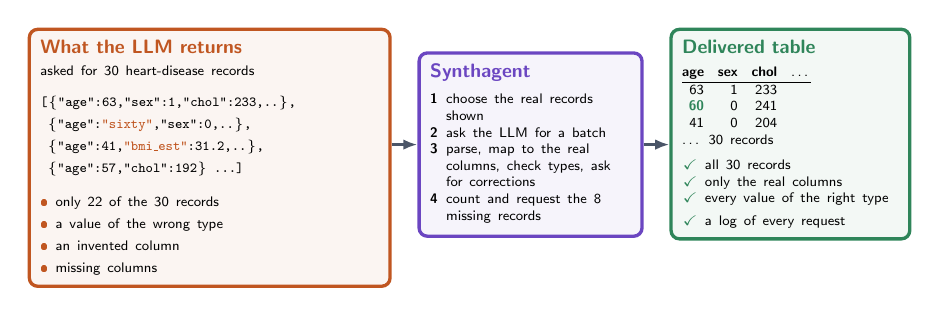
\begin{tikzpicture}[
  font=\sffamily\scriptsize,
  >={Latex[length=1.8mm]},
  box/.style={rounded corners=3pt,draw=#1,very thick,fill=#1!6,inner sep=4pt,align=left},
]
\providecommand{\bad}[1]{\textcolor{sorange}{\textbf{#1}}}
% ---------------- LLM response ----------------
\node[box=sorange,anchor=north west,text width=4.3cm] (raw) at (0,0) {%
  \textbf{\textcolor{sorange}{What the LLM returns}}\\
  {\tiny asked for 30 heart-disease records}\\[3pt]
  \texttt{\tiny [\{"age":63,"sex":1,"chol":233,..\},}\\
  \texttt{\tiny \ \{"age":\bad{"sixty"},"sex":0,..\},}\\
  \texttt{\tiny \ \{"age":41,\bad{"bmi\_est"}:31.2,..\},}\\
  \texttt{\tiny \ \{"age":57,"chol":192\} ...]}\\[4pt]
  {\tiny\bad{\textbullet} only 22 of the 30 records}\\
  {\tiny\bad{\textbullet} a value of the wrong type}\\
  {\tiny\bad{\textbullet} an invented column}\\
  {\tiny\bad{\textbullet} missing columns}};

% ---------------- Synthagent ----------------
\node[box=spurple,anchor=north west,text width=2.55cm] (ctl) at (4.95,-0.3) {%
  \textbf{\textcolor{spurple}{\system}}\\[3pt]
  {\tiny\setlength{\tabcolsep}{0pt}%
   \begin{tabular}{@{}l@{\hspace{3pt}}p{2.3cm}@{}}
   \textbf{1} & choose the real records shown\\
   \textbf{2} & ask the LLM for a batch\\
   \textbf{3} & parse, map to the real columns, check types, ask for corrections\\
   \textbf{4} & count and request the 8 missing records\\
   \end{tabular}}};

% ---------------- delivered table ----------------
\node[box=sgreen,anchor=north west,text width=2.75cm] (ok) at (8.15,0) {%
  \textbf{\textcolor{sgreen}{Delivered table}}\\[3pt]
  {\tiny\setlength{\tabcolsep}{2.5pt}%
   \begin{tabular}{@{}rrrc@{}}
   \textbf{age} & \textbf{sex} & \textbf{chol} & \dots\\\hline
   63 & 1 & 233 & \\
   \textcolor{sgreen}{\textbf{60}} & 0 & 241 & \\
   41 & 0 & 204 & \\
   \multicolumn{4}{@{}l}{\dots\ 30 records}\\
   \end{tabular}}\\[3pt]
  {\tiny\textcolor{sgreen}{\checkmark} all 30 records\\
   \textcolor{sgreen}{\checkmark} only the real columns\\
   \textcolor{sgreen}{\checkmark} every value of the right type\\
   \textcolor{sgreen}{\checkmark} a log of every request}};

\draw[->,very thick,sgray] (raw.east |- ctl.west) -- (ctl.west);
\draw[->,very thick,sgray] (ctl.east) -- (ok.west |- ctl.east);
\end{tikzpicture}
}
\caption{The problem addressed in this paper, in an illustrative example. Asked for 30 records of a heart-disease dataset, an LLM response (left) can contain too few records, invented or missing features and values of the wrong type. \system (right) validates and corrects every response, so the resulting dataset has the requested size and schema, and a log records each correction and its cost.}
\label{fig:teaser}
\end{figure}

%======================================================================
\section{Background \DIFdelbegin \DIFdel{and Related Work}\DIFdelend \DIFaddbegin \DIFadd{Knowledge}\DIFaddend }
\label{sec:related}
%======================================================================
\DIFdelbegin \DIFdel{To see where }%DIFDELCMD < \system %%%
\DIFdel{fits, we first review }\DIFdelend \DIFaddbegin \DIFadd{In this section, }\DIFaddend the families of \DIFdelbegin \DIFdel{tabular SDG methods , then examine what each family offers }\DIFdelend \DIFaddbegin \DIFadd{methods for synthetic data generation (SDG) of tabular data are first reviewed. Then, the limitations of each family }\DIFaddend when data are small \DIFaddbegin \DIFadd{are discussed}\DIFaddend , and finally \DIFdelbegin \DIFdel{consider }\DIFdelend the work on \DIFdelbegin \DIFdel{validated output and on the evaluation of synthetic dataon which our design and protocol build}\DIFdelend \DIFaddbegin \DIFadd{validating the output of LLMs and on evaluating synthetic data, on which }\system \DIFadd{builds, is presented}\DIFaddend .

\subsection{Synthetic Data Generation for Tabular Data}
Tabular SDG methods fall into four families\DIFdelbegin \DIFdel{. }\emph{\DIFdel{Interpolation and statistical models}} %DIFAUXCMD
\DIFdel{include SMOTE, which creates minority-class records on the }\DIFdelend \DIFaddbegin \DIFadd{, which differ in how they produce new records. }\emph{\DIFadd{Interpolation and statistical methods}} \DIFadd{derive new records directly from the real ones or from a simple probabilistic model of them: SMOTE places a new minority-class record on the line }\DIFaddend segment between two \DIFdelbegin \DIFdel{neighbours}\DIFdelend \DIFaddbegin \DIFadd{neighbouring records of that class}\DIFaddend ~\cite{chawla2002smote}, and Bayesian networks \DIFdelbegin \DIFdel{, which have also been used for differentially private release}\DIFdelend \DIFaddbegin \DIFadd{estimate the dependencies between features and sample new records from them}\DIFaddend ~\cite{zhang2014privbayes}. \emph{Deep generative models} \DIFdelbegin \DIFdel{learn the joint distribution with }\DIFdelend \DIFaddbegin \DIFadd{train }\DIFaddend a neural network \DIFdelbegin \DIFdel{: CTGAN and TVAE }\DIFdelend \DIFaddbegin \DIFadd{to approximate the joint distribution of the features and then sample from it: CTGAN trains a generator against a discriminator, TVAE learns a compressed representation of the records}\DIFaddend ~\cite{xu2019ctgan}, \DIFaddbegin \DIFadd{and }\DIFaddend diffusion models such as TabDDPM, CoDi and TabSyn \DIFdelbegin \DIFdel{~\mbox{%DIFAUXCMD
\cite{kotelnikov2023tabddpm,lee2023codi,zhang2024tabsyn}}\hskip0pt%DIFAUXCMD
, and }\DIFdelend \DIFaddbegin \DIFadd{learn to reverse a gradual corruption of the records~\mbox{%DIFAUXCMD
\cite{kotelnikov2023tabddpm,lee2023codi,zhang2024tabsyn}}\hskip0pt%DIFAUXCMD
; }\DIFaddend relational and cross-silo variants \DIFaddbegin \DIFadd{extend these models to several tables or institutions}\DIFaddend ~\cite{fan2020relational,shankar2024silofuse}. \emph{Fine-tuned language models} \DIFdelbegin \DIFdel{serialize }\DIFdelend \DIFaddbegin \DIFadd{write }\DIFaddend each record as \DIFdelbegin \DIFdel{text and }\DIFdelend \DIFaddbegin \DIFadd{a sentence, }\DIFaddend fine-tune a language model on \DIFdelbegin \DIFdel{the target data}\DIFdelend \DIFaddbegin \DIFadd{these sentences and generate new ones}\DIFaddend , as in GReaT~\cite{borisov2023great}, REaLTabFormer~\cite{solatorio2023realtabformer} and TabLoft~\cite{chen2026tabloft}. \emph{Prompted LLMs} \DIFdelbegin \DIFdel{generate records from examples placed }\DIFdelend \DIFaddbegin \DIFadd{place a few real records }\DIFaddend in the prompt \DIFdelbegin \DIFdel{, without }\DIFdelend \DIFaddbegin \DIFadd{of a pre-trained LLM and ask it for new ones, without any }\DIFaddend training, as in CLLM~\cite{seedat2024cllm} and EPIC~\cite{kim2024epic}.

\subsection{Synthetic Data Generation in Small Data}
Most of \DIFdelbegin \DIFdel{these }\DIFdelend \DIFaddbegin \DIFadd{the previously mentioned }\DIFaddend generators were designed and benchmarked on datasets with tens or hundreds of thousands of records, such as Adult (48,842 records) or Covertype (581,012 records)~\cite{xu2019ctgan}, and their behaviour on a few hundred records has received far less attention. \DIFdelbegin \DIFdel{Each familymeets small data with a different limitation, }\DIFdelend \DIFaddbegin \DIFadd{Table~\ref{tab:positioning} summarizes, for each family, how records are produced and its main limitation when data are small. Interpolation }\DIFaddend and \DIFdelbegin \DIFdel{naming the limitations makes clear which ones a new system must address. Interpolation methods and deep generators }\DIFdelend \DIFaddbegin \DIFadd{statistical methods, as well as deep generators, }\DIFaddend are fitted only to \DIFdelbegin \DIFdel{$D$; by the data-processing inequality~\mbox{%DIFAUXCMD
\cite{cover2006elements} }\hskip0pt%DIFAUXCMD
}\DIFdelend \DIFaddbegin \DIFadd{the real records, so }\DIFaddend they cannot add information \DIFdelbegin \DIFdel{about the task beyond what $D$ contains}\DIFdelend \DIFaddbegin \DIFadd{beyond what those records contain~\mbox{%DIFAUXCMD
\cite{cover2006elements}}\hskip0pt%DIFAUXCMD
}\DIFaddend , and they ignore what the features mean\DIFdelbegin \DIFdel{(L1, no external information)}\DIFdelend . Deep generators and fine-tuned language models must\DIFdelbegin \DIFdel{also }\DIFdelend \DIFaddbegin \DIFadd{, in addition, }\DIFaddend estimate many parameters from few records, so they can produce records outside the observed ranges and types, or reproduce training records~\cite{hyeong2022tabularmia}\DIFdelbegin \DIFdel{(L2, training on scarce records)}\DIFdelend . Prompted LLMs \DIFdelbegin \DIFdel{avoid both problems}\DIFdelend \DIFaddbegin \DIFadd{need no training and bring domain knowledge}\DIFaddend , but nothing ensures that their output is a valid dataset of the requested size, and its cost is not measured\DIFdelbegin \DIFdel{(L3, unreliable output)}\DIFdelend ; CLLM~\cite{seedat2024cllm} filters \DIFaddbegin \DIFadd{the }\DIFaddend generated records by their learning dynamics and EPIC~\cite{kim2024epic} designs balanced prompts, but both concern the quality of the records that are kept rather than the size, validity and cost of the output. Across all families, finally, generators are usually compared \DIFdelbegin \DIFdel{from single runs}\DIFdelend \DIFaddbegin \DIFadd{on a single run}\DIFaddend , so differences caused by \DIFdelbegin \DIFdel{run-to-run variation }\DIFdelend \DIFaddbegin \DIFadd{the variation between runs}\DIFaddend , which is large in small data, are reported as effects\DIFdelbegin \DIFdel{(L4, evaluation without a noise estimate)}\DIFdelend . \system \DIFdelbegin \DIFdel{addresses L3 }\DIFdelend \DIFaddbegin \DIFadd{targets the limitation of prompted LLMs }\DIFaddend with its control layer \DIFdelbegin \DIFdel{and L4 with its evaluation protocol, and , because it uses }\DIFdelend \DIFaddbegin \DIFadd{while keeping their advantages, and its evaluation measures the variation between repeated runs before comparing configurations.
}

\begin{table*}[t]
\centering
\caption{\DIFaddFL{Families of tabular SDG methods: how they produce records, their main limitation in small data, and their properties. }\checkmark\DIFaddFL{: by design; (}\checkmark\DIFaddFL{): partially (SMOTE's number of records follows the class balance; fine-tuned language models discard unreadable records); $\times$: not addressed.}}
\label{tab:positioning}
\footnotesize
\setlength{\tabcolsep}{3pt}
\begin{tabular}{@{}p{.15\textwidth}p{.23\textwidth}p{.27\textwidth}cccc@{}}
\toprule
Family & How records are produced & Main limitation in small data & \begin{tabular}[c]{@{}c@{}}No training on\\target data\end{tabular} & \begin{tabular}[c]{@{}c@{}}Exact\\size\end{tabular} & \begin{tabular}[c]{@{}c@{}}Columns and\\types checked\end{tabular} & \begin{tabular}[c]{@{}c@{}}Cost\\recorded\end{tabular} \\
\midrule
\DIFaddFL{Interpolation and statistical~\mbox{%DIFAUXCMD
\cite{chawla2002smote,zhang2014privbayes} }\hskip0pt%DIFAUXCMD
}& \DIFaddFL{Combine real records or sample a simple model fitted to them }& \DIFaddFL{Only recombine existing patterns; ignore feature meaning }& \checkmark & \DIFaddFL{(}\checkmark\DIFaddFL{) }& \DIFaddFL{$\times$ }& \DIFaddFL{$\times$ }\\
\DIFaddFL{Deep generative~\mbox{%DIFAUXCMD
\cite{xu2019ctgan,kotelnikov2023tabddpm,zhang2024tabsyn} }\hskip0pt%DIFAUXCMD
}& \DIFaddFL{Train a neural network on the real records and sample from it }& \DIFaddFL{Few records to fit many parameters; invalid or copied records }& \DIFaddFL{$\times$ }& \checkmark & \DIFaddFL{$\times$ }& \DIFaddFL{$\times$ }\\
\DIFaddFL{Fine-tuned language models~\mbox{%DIFAUXCMD
\cite{borisov2023great,solatorio2023realtabformer} }\hskip0pt%DIFAUXCMD
}& \DIFaddFL{Fine-tune a language model on records written as text }& \DIFaddFL{Training on scarce records }& \DIFaddFL{$\times$ }& \checkmark & \DIFaddFL{(}\checkmark\DIFaddFL{) }& \DIFaddFL{$\times$ }\\
\DIFaddFL{Prompted LLMs~\mbox{%DIFAUXCMD
\cite{seedat2024cllm,kim2024epic} }\hskip0pt%DIFAUXCMD
}& \DIFaddFL{Ask }\DIFaddendFL a pre-trained LLM \DIFdelbeginFL \DIFdelFL{, it inherits the advantages of prompted LLMs over L1 and L2. Table~\ref{tab:positioning} summarizes these differences. The next subsection explains where the idea of }\DIFdelendFL \DIFaddbeginFL \DIFaddFL{for records, with real examples in the prompt }& \DIFaddFL{Unreliable output: wrong size, malformed records, unknown cost }& \checkmark & \DIFaddFL{$\times$ }& \DIFaddFL{$\times$ }& \DIFaddFL{$\times$ }\\
\midrule
\system \DIFaddFL{(ours) }& \DIFaddFL{Prompted LLM whose output is checked and completed by }\DIFaddendFL a control layer \DIFdelbeginFL \DIFdelFL{comes from.
}%DIFDELCMD < 

%DIFDELCMD < \begin{table}[t]
%DIFDELCMD < \centering
%DIFDELCMD < %%%
%DIFDELCMD < \caption{%
{%DIFAUXCMD
\DIFdelFL{Properties of existing generator families and of }%DIFDELCMD < \system%%%
\DIFdelFL{. }%DIFDELCMD < \checkmark%%%
\DIFdelFL{: by design; (}%DIFDELCMD < \checkmark%%%
\DIFdelFL{): partially (SMOTE's size follows the class balance; fine-tuned LMs discard unparsable records); $\times$: not addressed.}}
%DIFAUXCMD
%DIFDELCMD < \label{tab:positioning}
%DIFDELCMD < \footnotesize
%DIFDELCMD < \setlength{\tabcolsep}{1.5pt}
%DIFDELCMD < \begin{tabular*}{\columnwidth}{@{\extracolsep{\fill}}lcccc@{}}
%DIFDELCMD < \toprule
%DIFDELCMD < Family & \begin{tabular}[c]{@{}c@{}}No training\\on $D$\end{tabular} & \begin{tabular}[c]{@{}c@{}}Exact\\size\end{tabular} & \begin{tabular}[c]{@{}c@{}}Schema\\validated\end{tabular} & \begin{tabular}[c]{@{}c@{}}Cost\\measured\end{tabular} \\
%DIFDELCMD < \midrule
%DIFDELCMD < Interpolation~\cite{chawla2002smote} & \checkmark & (\checkmark) & $\times$ & $\times$ \\
%DIFDELCMD < Deep generators~\cite{xu2019ctgan,kotelnikov2023tabddpm,zhang2024tabsyn} & $\times$ & \checkmark & $\times$ & $\times$ \\
%DIFDELCMD < Fine-tuned LMs~\cite{borisov2023great,solatorio2023realtabformer} & $\times$ & \checkmark & (\checkmark) & $\times$ \\
%DIFDELCMD < Prompted LLMs~\cite{seedat2024cllm,kim2024epic} & \checkmark & $\times$ & $\times$ & $\times$ \\
%DIFDELCMD < \midrule
%DIFDELCMD < \system (ours) & \checkmark & \checkmark & \checkmark & \checkmark \\
%DIFDELCMD < \bottomrule
%DIFDELCMD < \end{tabular*}
%DIFDELCMD < \end{table}
%DIFDELCMD < %%%
\DIFdelendFL \DIFaddbeginFL & \DIFaddFL{--- }& \checkmark & \checkmark & \checkmark & \checkmark \\
\bottomrule
\end{tabular}
\end{table*}
\DIFaddend 

\subsection{LLM Agents, Validated Output and Data Quality}
The control layer \DIFaddbegin \DIFadd{of }\system\DIFadd{, introduced in Section~\ref{sec:intro}, }\DIFaddend follows the agent pattern of alternating actions and observations~\cite{yao2023react,wang2024agentsurvey}, but its observations are deterministic checks \DIFaddbegin \DIFadd{of the output of the LLM }\DIFaddend rather than the model's own reflections. This choice connects \system to a long line of data-management work. Synthetic data have long been used to test systems and share data~\cite{sanghi2023enterprise,fan2020relational}; Kamino enforces denial constraints during private synthesis~\cite{ge2021kamino}; data-cleaning systems combine statistical inference with integrity constraints~\cite{chu2013holistic,qin2024bclean}; foundation models can clean and integrate data through prompting~\cite{narayan2022wrangle}; and recovering structured records from free-form LLM output is a data-engineering problem in its own right~\cite{rorseth2026recovering}. \system applies the same principle to generation: the schema and type rules are inferred from the data, and every response is parsed and validated against them. Unlike feature augmentation, which adds columns from related tables~\cite{liang2025featpilot}, it adds records.

\subsection{Evaluating Synthetic Data}
Data-preparation studies have shown that a step that looks beneficial can harm downstream models~\cite{li2021cleanml,guha2023cleaningfairness}, and evaluation frameworks such as Synthcity and SynthEval recommend assessing fidelity, privacy and utility together~\cite{qian2023synthcity,lautrup2025syntheval}. Fidelity can be complemented by a classifier two-sample test, which asks whether a classifier can tell real from synthetic records~\cite{lopezpaz2017c2st}, and privacy by membership-inference attacks, which ask whether an attacker can tell which records were used for generation~\cite{shokri2017mia,hyeong2022tabularmia}. Formal guarantees require syntactic anonymization models such as $\ell$-diversity and $t$-closeness~\cite{machanavajjhala2006ldiversity,li2007tcloseness} or differential privacy~\cite{dwork2014dp}, which \system does not claim. Our protocol (Section~\ref{sec:setup}) adopts the multi-dimensional view and adds the paired comparison and noise estimate that small data requires.

%======================================================================
\section{Problem Formulation}
\label{sec:problem}
%======================================================================
We now state the problem introduced in Section~\ref{sec:intro} precisely. Given a small dataset $D$, its schema $S$ (the features and their types) and a requested number of synthetic records $N$, the goal is to produce, without training a generator on $D$, a synthetic dataset $G$ that satisfies six requirements: it has exactly $N$ records (R1); every record conforms to $S$ (R2); the cost of producing it is measured (R3); it is faithful to the distribution of $D$ (R4); it does not reproduce the records of $D$ (R5); and adding it to the training data improves, or at least does not degrade, the classifiers trained on $D$ (R6). \DIFdelbegin \DIFdel{The first three requirements describe a dependable dataset and can be guaranteed by a system ; the last three describe a useful one and }\DIFdelend \DIFaddbegin \DIFadd{These requirements are not new; they combine two established lines of work. R1 to R3 correspond to data-quality dimensions used in data management, namely completeness, conformity to a schema and the cost of acquiring the data~\mbox{%DIFAUXCMD
\cite{wang1996beyond,batini2009methodologies}}\hskip0pt%DIFAUXCMD
, and they concern the synthetic dataset as a data product: a system can guarantee them. R4 to R6 are the three dimensions on which synthetic data are evaluated in the literature, namely fidelity, privacy and utility~\mbox{%DIFAUXCMD
\cite{qian2023synthcity,lautrup2025syntheval}}\hskip0pt%DIFAUXCMD
, and they concern the value of the synthetic records: they }\DIFaddend can only be measured. \DIFaddbegin \DIFadd{The relation between the two groups is therefore one of order. A dataset that fails R1 or R2 cannot be used at all, so its fidelity, privacy and utility are not even defined, whereas a dataset that satisfies R1 to R3 can then be judged on R4 to R6. }\DIFaddend Formally, let $D^{\mathrm{tr}}$ and $D^{\mathrm{te}}$ be a training and a test partition of a small dataset $D$ with schema $S$, and let a configuration $\theta$ of the system (LLM, context strategy, active rules) produce a synthetic dataset $G_\theta$ from $D^{\mathrm{tr}}$ without access to $D^{\mathrm{te}}$. Requirements R1 and R2 define the feasible set $\mathcal{F}(S,R,N)$ of datasets with exactly $N$ records that conform to $S$ and to the active rules $R$. The other requirements are objectives: a fidelity loss $L_{\mathrm{fid}}(D^{\mathrm{tr}},G_\theta)$ for R4, a privacy risk $L_{\mathrm{priv}}(D^{\mathrm{tr}},G_\theta)$ for R5, the change in downstream utility $\Delta U(G_\theta)$ for R6 and the generation cost $\kappa(\theta)$, which R3 requires to be measured and which should also be kept low:
\begin{equation}
\theta^{\star}\in\operatorname*{arg\,min}_{\theta:\,G_{\theta}\in\mathcal{F}(S,R,N)}
\bigl(L_{\mathrm{fid}},\;L_{\mathrm{priv}},\;-\Delta U,\;\kappa\bigr)(\theta).
\label{eq:multiobjective}
\end{equation}
The objectives in Equation~\eqref{eq:multiobjective} can conflict: records closer to the real ones are more faithful but easier to attack, and a larger LLM may produce better records at a higher cost. We therefore do not collapse them into one weighted score, because the right weights depend on the use; a healthcare facility sharing data for software testing weights privacy and validity, whereas a team augmenting a classifier weights utility. The formulation also divides the work of the paper. The constraint $G_\theta\in\mathcal{F}(S,R,N)$ is the responsibility of the system, which the next section describes; the objectives are the subject of the evaluation that follows it.

%======================================================================
\section{The \system System}
\label{sec:system}
%======================================================================
\system meets the constraint of Equation~\eqref{eq:multiobjective} by \DIFdelbegin \DIFdel{never trusting the LLM with it. }\DIFdelend \DIFaddbegin \DIFadd{checking the output of the LLM instead of relying on it: every response is verified, and corrected or completed when necessary, before its records enter the synthetic dataset. The architecture that implements this principle is shown in }\DIFaddend Figure~\ref{fig:architecture}\DIFdelbegin \DIFdel{shows the architecture}\DIFdelend . A profiling step infers the schema $S$ and the type rules $R$ from the training data. Each request then passes through four stages: the context selector builds the prompt (1), the LLM proposes a batch of records (2), the parser and validator check it (3), and the accepted records are counted against the requested size (4). Each type of failure triggers its own correction. We describe first the state that ties these stages together and then each stage in turn.

\begin{figure*}[t]
\centering
\resizebox{\textwidth}{!}{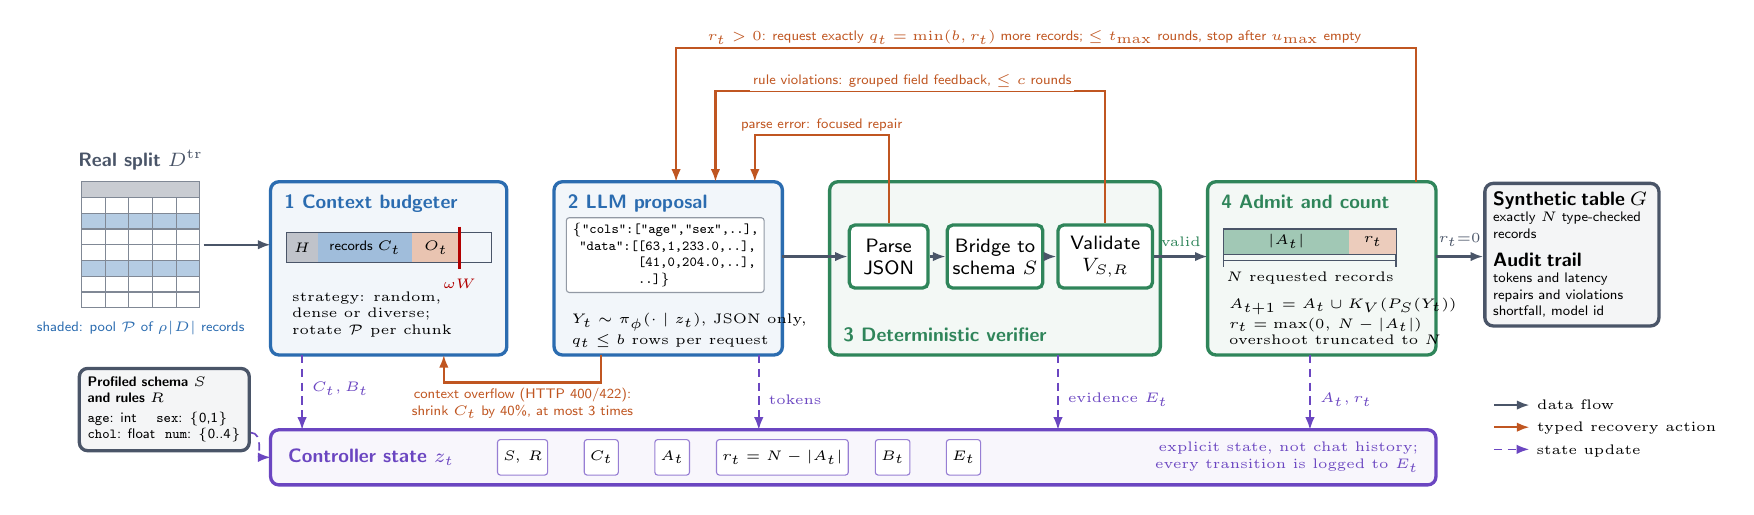
\begin{tikzpicture}[
  font=\sffamily\scriptsize,
  >={Latex[length=1.6mm]},
  flow/.style={->,thick,sgray},
  fail/.style={->,thick,sorange},
  st/.style={->,densely dashed,spurple,semithick},
  pan/.style={rounded corners=3pt,draw=#1,very thick,fill=#1!6},
  ttl/.style={font=\sffamily\bfseries\scriptsize,text=#1,anchor=north west},
  gate/.style={draw=sgreen,very thick,fill=white,rounded corners=2pt,minimum height=8mm,align=center,inner sep=2pt},
  lab/.style={font=\sffamily\tiny,text=#1,fill=white,inner sep=1pt},
]
%======================== panels ========================
\draw[pan=sblue]   (2.4,0) rectangle (5.4,-2.2);   \node[ttl=sblue]  at (2.45,-0.05) {1\,\,Context budgeter};
\draw[pan=sblue]   (6.0,0) rectangle (8.9,-2.2);   \node[ttl=sblue]  at (6.05,-0.05) {2\,\,LLM proposal};
\draw[pan=sgreen]  (9.5,0) rectangle (13.7,-2.2);  \node[ttl=sgreen,anchor=south west] at (9.55,-2.15) {3\,\,Deterministic verifier};
\draw[pan=sgreen]  (14.3,0) rectangle (17.2,-2.2); \node[ttl=sgreen] at (14.35,-0.05) {4\,\,Admit and count};

%======================== real data =====================
\foreach \r in {1,...,7}{\foreach \c in {0,...,4}{
   \ifnum\r=2 \fill[sblue!35] (\c*0.3,-\r*0.2) rectangle ++(0.3,-0.2);\fi
   \ifnum\r=5 \fill[sblue!35] (\c*0.3,-\r*0.2) rectangle ++(0.3,-0.2);\fi
   \draw[sgray!70] (\c*0.3,-\r*0.2) rectangle ++(0.3,-0.2);}}
\fill[sgray!30] (0,0) rectangle (1.5,-0.2); \draw[sgray!70] (0,0) rectangle (1.5,-0.2);
\node[font=\sffamily\bfseries\scriptsize,text=sgray,anchor=south] at (0.75,0.02) {Real split $D^{\mathrm{tr}}$};
\node[font=\sffamily\tiny,text=sblue,align=center,anchor=north] at (0.75,-1.65) {shaded: pool $\mathcal{P}$ of $\rho|D|$ records};
\draw[flow] (1.55,-0.8) -- (2.4,-0.8);

% profile card
\node[pan=sgray,anchor=north west,align=left,inner sep=3pt,font=\sffamily\tiny] (prof) at (-0.05,-2.35)
  {\textbf{Profiled schema $S$}\\\textbf{and rules $R$}\\[1pt]
   \texttt{age}: int \quad \texttt{sex}: \{0,1\}\\ \texttt{chol}: float \ \texttt{num}: \{0..4\}};

%======================== 1 budgeter ====================
\begin{scope}[shift={(2.6,-0.65)}]
  \fill[sgray!35]   (0,0) rectangle (0.4,-0.38);  \node at (0.2,-0.19)  {\tiny $H$};
  \fill[sblue!45]   (0.4,0) rectangle (1.6,-0.38); \node at (1.0,-0.19) {\tiny records $C_t$};
  \fill[sorange!35] (1.6,0) rectangle (2.2,-0.38); \node at (1.9,-0.19) {\tiny $O_t$};
  \draw[sgray] (0,0) rectangle (2.6,-0.38);
  \draw[red!70!black,thick] (2.2,0.08) -- (2.2,-0.46);
  \node[font=\tiny,text=red!70!black,anchor=north] at (2.2,-0.46) {$\omega W$};
  \node[font=\tiny,anchor=north west,align=left] at (-0.05,-0.62)
     {strategy: random,\\dense or diverse;\\rotate $\mathcal{P}$ per chunk};
\end{scope}

%======================== 2 LLM =========================
\node[anchor=north west,draw=sgray!60,fill=white,rounded corners=1pt,align=left,font=\ttfamily\tiny,inner sep=2pt]
  at (6.15,-0.45)
  {\{"cols":["age","sex",..],\\ \ "data":[[63,1,233.0,..],\\ \hphantom{\ "data":[}[41,0,204.0,..],\\ \hphantom{\ "data":[}..]\}};
\node[font=\tiny,anchor=north west,align=left] at (6.1,-1.55) {$Y_t\sim\pi_\phi(\cdot\mid z_t)$, JSON only,\\ $q_t\le b$ rows per request};

%======================== 3 verifier ====================
\node[gate,minimum width=10mm] (g1) at (10.25,-0.95) {Parse\\JSON};
\node[gate,minimum width=12mm] (g2) at (11.6,-0.95)  {Bridge to\\schema $S$};
\node[gate,minimum width=12mm] (g3) at (13.0,-0.95)  {Validate\\$V_{S,R}$};
\draw[flow] (g1)--(g2); \draw[flow] (g2)--(g3);
\draw[flow] (8.9,-0.95) -- (g1.west);

%======================== 4 admit =======================
\begin{scope}[shift={(14.5,-0.6)}]
  \fill[sgreen!45]  (0,0) rectangle (1.6,-0.32);
  \fill[sorange!30] (1.6,0) rectangle (2.2,-0.32);
  \draw[sgray] (0,0) rectangle (2.2,-0.32);
  \node at (0.8,-0.16) {\tiny $|A_t|$}; \node at (1.9,-0.16) {\tiny $r_t$};
  \draw[sgray,|-|] (0,-0.4) -- (2.2,-0.4);
  \node[font=\tiny,anchor=north] at (1.1,-0.42) {$N$ requested records};
  \node[font=\tiny,anchor=north west,align=left] at (-0.05,-0.75)
    {$A_{t+1}=A_t\cup K_V(P_S(Y_t))$\\$r_t=\max(0,\,N-|A_t|)$\\overshoot truncated to $N$};
\end{scope}
\draw[flow] (g3.east) -- node[above,font=\tiny,text=sgreen]{valid} (14.3,-0.95);

%======================== output ========================
\node[pan=sgray,anchor=north west,align=left,inner sep=3pt,text width=20mm,font=\sffamily\tiny] (out) at (17.8,0)
  {\textbf{\scriptsize Synthetic table $G$}\\exactly $N$ type-checked records\\[4pt]\textbf{\scriptsize Audit trail}\\tokens and latency\\repairs and violations\\shortfall, model id};
\draw[flow] (17.2,-0.95) -- node[above,font=\tiny]{$r_t{=}0$} (out.west|-0,-0.95);

%======================== recovery loops ================
% parse error -> focused repair
\draw[fail] (g1.north) -- (10.25,0.6) -- (8.55,0.6) -- (8.55,0);
\node[lab=sorange,anchor=south] at (9.4,0.6) {parse error: focused repair};
% violations -> grouped feedback
\draw[fail] (g3.north) -- (13.0,1.15) -- (8.05,1.15) -- (8.05,0);
\node[lab=sorange,anchor=south] at (10.55,1.15) {rule violations: grouped field feedback, $\le c$ rounds};
% residual -> top-up
\draw[fail] (16.95,0) -- (16.95,1.7) -- (7.55,1.7) -- (7.55,0);
\node[lab=sorange,anchor=south] at (12.1,1.7) {$r_t>0$: request exactly $q_t=\min(b,r_t)$ more records; $\le t_{\max}$ rounds, stop after $u_{\max}$ empty};
% overflow -> shrink context (below)
\draw[fail] (6.6,-2.2) -- (6.6,-2.55) -- (4.6,-2.55) -- (4.6,-2.2);
\node[lab=sorange,anchor=north,align=center] at (5.6,-2.58) {context overflow (HTTP 400/422):\\shrink $C_t$ by 40\%, at most 3 times};

%======================== state register ================
\draw[draw=spurple,very thick,fill=spurple!5,rounded corners=3pt] (2.4,-3.15) rectangle (17.2,-3.85);
\node[font=\sffamily\bfseries\scriptsize,text=spurple,anchor=west] at (2.5,-3.5) {Controller state $z_t$};
\foreach \lab/\x in {{$S,\,R$}/5.6,{$C_t$}/6.6,{$A_t$}/7.5,{$r_t=N-|A_t|$}/8.9,{$B_t$}/10.3,{$E_t$}/11.2}{
  \node[draw=spurple!70,fill=white,rounded corners=1pt,minimum height=4.5mm,inner sep=2pt,font=\tiny] at (\x,-3.5) {\lab};}
\node[font=\tiny,text=spurple,anchor=east,align=right] at (17.1,-3.5) {explicit state, not chat history;\\every transition is logged to $E_t$};
\draw[st] (prof.south east) ++(0,0.25) to[out=0,in=180] (2.4,-3.5);
\draw[st] (2.8,-2.2) -- (2.8,-3.15) node[pos=.45,right,font=\tiny]{$C_t,B_t$};
\draw[st] (8.6,-2.2) -- (8.6,-3.15) node[pos=.6,right,font=\tiny]{tokens};
\draw[st] (12.4,-2.2) -- (12.4,-3.15) node[pos=.6,right,font=\tiny]{evidence $E_t$};
\draw[st] (15.6,-2.2) -- (15.6,-3.15) node[pos=.6,right,font=\tiny]{$A_t,r_t$};

%======================== legend ========================
\node[anchor=north west,font=\tiny,align=left] at (17.8,-2.65) {
  \tikz\draw[flow](0,0)--(0.45,0); data flow\\[2pt]
  \tikz\draw[fail](0,0)--(0.45,0); typed recovery action\\[2pt]
  \tikz\draw[st](0,0)--(0.45,0); state update};
\end{tikzpicture}
}
\caption{Architecture of \system. Real records enter a context window of limited size (1); the LLM proposes a JSON batch (2); deterministic checks parse it, map it to the schema and validate the type rules (3); and accepted records are counted against the requested size (4). Each failure type triggers its own correction (orange). Every stage reads or updates the state $z_t$ of the control layer (purple), which also serves as the audit log of the run.}
\label{fig:architecture}
\end{figure*}

\subsection{State of the Control Layer}
Let $N$ be the requested number of synthetic records and $R$ the active rules. At step $t$, the control layer keeps the state
\begin{equation}
z_t=(S,\,R,\,C_t,\,A_t,\,N-|A_t|,\,B_t,\,E_t),
\label{eq:state}
\end{equation}
where $C_t$ is the set of real records shown to the LLM, $A_t$ the accepted synthetic records, $N-|A_t|$ the number still missing, $B_t$ the remaining token budget and $E_t$ the log of parser and validator results. The LLM, denoted $\pi_{\phi}$, proposes a batch $Y_t\sim\pi_{\phi}(\cdot\mid z_t)$. Let $P_S$ be the parser, which also maps the returned features to $S$, $V_{S,R}$ the validator and $K$ a correction step that sends invalid values back to the LLM, at most twice. The accepted set is updated as
\begin{equation}
A_{t+1}=A_t\cup K_{V_{S,R}}\bigl(P_S(Y_t)\bigr).
\label{eq:acceptance}
\end{equation}
Equation~\eqref{eq:acceptance} expresses the central design decision: the LLM only proposes, and a record enters $A_{t+1}$ only after it has been parsed, mapped to $S$ and validated. Because the state is explicit rather than implied by the conversation history, the number of missing records is always known, and $E_t$ records every failure for later inspection. The remaining subsections describe how each component reads and updates this state.

\subsection{Context Selection (R1, R3)}
The context selector decides which real records the LLM sees. Table~\ref{tab:prompt-context} lists exactly what the model receives in our experiments. The core evidence is a 20\% sample of the real training split, serialized as compact row-major JSON with the ordered feature columns and the observed target, so the model sees how features and class co-occur in real records. No free-text description of the \DIFdelbegin \DIFdel{clinical }\DIFdelend \DIFaddbegin \DIFadd{prediction }\DIFaddend task is added, so that no dataset receives more prompt engineering than another; the model must infer the role of each feature from its name and values.

\begin{table*}[t]
\centering
\caption{Information boundary for one generation request in the reported study. ``Not supplied'' is intentional: those signals cannot influence the generated records.}
\label{tab:prompt-context}
\DIFdelbeginFL %DIFDELCMD < \small
%DIFDELCMD < %%%
\DIFdelendFL \DIFaddbeginFL \footnotesize
\DIFaddendFL \begin{tabular}{p{.17\textwidth}p{.36\textwidth}p{.39\textwidth}}
\toprule
Context layer & What the model receives & Why it is included or excluded \\
\midrule
Schema & Ordered column names and an exact column-count requirement & Fixes the record interface and prevents invented or omitted fields. \\
Demonstrations & Compact row-major serialization of a 20\% sample of the training records, with feature and target values & Exposes joint patterns, value formats, label prevalence and plausible cross-column combinations without sending the whole local table. \\
Generation task & Exact number of new records for the current batch, at most 30 & Turns an open-ended completion into a bounded action whose output count can be verified. \\
Output contract & JSON only, fixed column order, complete cells, raw numeric values, no extra metadata & Makes parsing deterministic and removes interface failures unrelated to statistical quality. \\
Dynamic feedback & Parser error location after malformed JSON, or grouped field violations after failed validation & Reveals only the evidence needed for a targeted repair instead of replaying the full history. \\
Free-text metadata & Not supplied & Prevents unequal, dataset-specific prompt engineering from confounding the comparison. \\
Test information & No holdout rows, predictions, metrics or classifier identities & Preserves the evaluation boundary and prevents optimization against the test set. \\
Global statistics & No separately computed means, quantiles, correlations or class quotas & Fidelity must arise from the selected records; the consequence is weaker protection against rare-mode omission. \\
\bottomrule
\end{tabular}
\end{table*}

Formally, a selection strategy $s\in\{\text{random},\text{dense},\text{diverse}\}$ defines an ordered candidate pool, and the token budget determines how much of that pool is visible:
\begin{equation}
\begin{aligned}
C_t&=\operatorname{Slice}_{t}\!\left(\operatorname{Select}_{s}
(D^{\mathrm{tr}},\lceil0.2|D^{\mathrm{tr}}|\rceil),k_t\right),\\
k_t&=\max\{k:T(H,I,C_{t,k},O_t)\leq0.85W\}.
\end{aligned}
\label{eq:context}
\end{equation}
Here $H$ is the schema and output contract, $I$ optional instruction text, $O_t$ the reserved output, $W$ the backend context window and $T$ a token estimator (2.8 characters per token for compact JSON). The slice operator rotates through the pool across chunks, so successive requests see different patients when the pool exceeds one window. If the provider still rejects a request as too long (HTTP 400 or 422), the control layer shrinks the visible context by 40\% and retries, at most three times. ``20\% context'' therefore describes the candidate pool, not a promise that every candidate row appears in every prompt.

The 20\% fraction and the 85\% window limit were fixed before the experiments and not tuned. The default strategy samples the context at random. \emph{Dense} prefers records with the most observed cells, reducing ambiguity from missing fields. \emph{Diverse} standardizes numerical features, runs $k$-means and selects the records nearest to the centroids, so that the context covers more of the feature space. Neither strategy is class-stratified, so neither guarantees that a rare diagnosis appears in context; Section~\ref{sec:discussion} returns to this limitation.

\subsection{Parsing, Validation and Correction (R2)}
The parser and the validator decide which parts of a response can enter the accepted set $A_t$ of Equation~\eqref{eq:acceptance}.
Records are requested in JSON batches of at most 30, a size that keeps every response within the output limit of the smallest LLM tested and limits the loss when a response fails. A local parser first extracts structured content and fixes common defects (non-finite literals, trailing commas, concatenated objects). If parsing still fails, the control layer issues one repair request at temperature 0.1 that quotes the error position and surrounding text. The returned feature names are then mapped back to the schema.

Profiling infers a type rule for every feature, and optional boundary rules (numerical ranges with 10\% tolerance, or categorical domains with at most 20 values). Dynamic Pydantic models validate each batch. The validator groups failures by field and reports one representative bad value per field, so the correction prompt does not grow linearly with repeated errors. Up to two correction rounds are attempted per batch. User-defined post-processing rules (noise, rounding, normalization) can be applied deterministically afterwards.

In the reference configuration of our experiments, type rules are active, boundary rules are off and no user rules are supplied, so we evaluate the default system rather than the strictest one. Rules are used only by the validator and are never inserted into the prompt.

\subsection{Completion Loop (R1)}
LLMs often return fewer records than requested, as RQ1 will show. The completion loop derives its next request from the accepted state rather than from the conversation:
\begin{equation}
r_t=\max(0,N-|A_t|),\qquad q_t=\min(30,r_t).
\label{eq:residual}
\end{equation}
Equation~\eqref{eq:residual} requests only the residual $q_t$, and any overshoot is truncated. The loop runs for at most 50 top-up rounds and stops after five consecutive empty or unparsable responses. Successful runs therefore return exactly $N$ records; persistent provider failure can still end a run short, and that shortfall is recorded rather than hidden. Algorithm~\ref{alg:loop} summarizes the complete loop.

\begin{algorithm}[t]
\caption{Generation loop of the control layer}
\label{alg:loop}
\small
\begin{algorithmic}[1]
\Require training records $D^{\mathrm{tr}}$, schema $S$, rules $R$, size $N$, strategy $s$, window $W$
\State $\mathcal{P}\gets\operatorname{Select}_s(D^{\mathrm{tr}},\lceil0.2|D^{\mathrm{tr}}|\rceil)$; $A\gets\emptyset$; $E\gets[\,]$
\For{chunk $t=1,\dots,\lceil N/30\rceil$}
  \State $C_t\gets$ rotated slice of $\mathcal{P}$ that fits $0.85W$ \Comment{Eq.~\eqref{eq:context}}
  \State $Y\gets\pi_\phi(S,C_t,\min(30,N-30(t-1)))$; on overflow shrink $C_t$ by 40\%, retry $\le3$
  \State $X\gets P_S(Y)$; \textbf{if} parse fails \textbf{then} $X\gets P_S(\text{repair}(Y))$
  \For{$j=1,2$} \Comment{targeted correction}
    \State \textbf{if} $V_{S,R}(X)$ has no violations \textbf{then break}
    \State $X\gets P_S(\pi_\phi(\text{grouped violations of }X))$; append to $E$
  \EndFor
  \State $A\gets A\cup X$
\EndFor
\State $u\gets0$
\While{$|A|<N$ \textbf{and} fewer than 50 rounds \textbf{and} $u<5$} \Comment{Eq.~\eqref{eq:residual}}
  \State $X\gets P_S(\pi_\phi(S,\text{first 20 records of }\mathcal{P},\min(30,N-|A|)))$
  \State \textbf{if} $X=\emptyset$ \textbf{then} $u\gets u+1$ \textbf{else} $A\gets A\cup X$; $u\gets0$
\EndWhile
\State \Return first $N$ rows of $A$, together with $E$, token counts and timings
\end{algorithmic}
\end{algorithm}

The last element of the control layer is its audit log, which serves R3. Every run records prompt, completion and total tokens, LLM generation time, parser repair attempts, rule violations, the requested and delivered record counts and the model identifier. These records make a synthetic dataset inspectable after the fact and give the cost term $\kappa(\theta)$ in Equation~\eqref{eq:multiobjective} a measured value.


\subsection{Deployment Across Healthcare Facilities}
\label{sec:deployment}
The setting that motivates this work, small datasets held by healthcare facilities that cannot pool them~\cite{rieke2020digitalhealth,sheller2020medicine}, also suggests how \system can be deployed. Because the control layer needs only a local dataset, its schema and an inference endpoint, each healthcare facility of a network can run it inside its own infrastructure. Consider $K$ healthcare facilities, each holding a small dataset $D_k$ for the same prediction task, with different case mix, coding practice and class prevalence. Each healthcare facility runs \system locally and trains on its real and synthetic records,
\begin{equation}
G_k=\mathcal{A}(D_k,S_k,R_k,B_k),\qquad
\Delta w_k=\mathcal{U}(w_t,D_k\cup G_k),
\label{eq:local-federated}
\end{equation}
where $S_k$ and $R_k$ are the local schema and rules, $B_k$ the local token budget and $\mathcal{U}$ the local training procedure. Only the model update $\Delta w_k$ and approved aggregate diagnostics leave the healthcare facility. A coordinator aggregates the updates as in FedAvg~\cite{mcmahan2017fedavg,kairouz2021federated},
\begin{equation}
w_{t+1}=w_t+\sum_{k\in\mathcal{K}_t}\frac{n_k}{\sum_{j\in\mathcal{K}_t}n_j}\,\Delta w_k,\qquad n_k=|D_k|,
\label{eq:federated-aggregate}
\end{equation}
preferably under secure aggregation~\cite{bonawitz2017secure}. The weights count \emph{real} records, $|D_k|$ rather than $|D_k\cup G_k|$, so a healthcare facility gains no extra weight by generating more records (Figure~\ref{fig:federated}). Unlike SiloFuse, which trains a shared generator across sites~\cite{shankar2024silofuse}, this design needs no generator training across healthcare facilities, and each healthcare facility can reject its synthetic records when paired local validation shows no gain. The design is not, by itself, a privacy guarantee: with a remote LLM the prompt content leaves the healthcare facility, so sensitive deployments need a locally served model or a data-processing agreement, and both synthetic records and model updates can leak information~\cite{chen2024modeltrip}. Our experiments evaluate the generation step one healthcare facility at a time, which is the setting the next section describes; a multi-site evaluation is future work.



\begin{figure*}[t]
\centering
\begin{minipage}[c]{0.6\textwidth}
\resizebox{\linewidth}{!}{% Cross-silo deployment figure (Fig. fig:federated). Requires TikZ libraries
% arrows.meta, calc, shapes.geometric and the s* colours from main.tex.
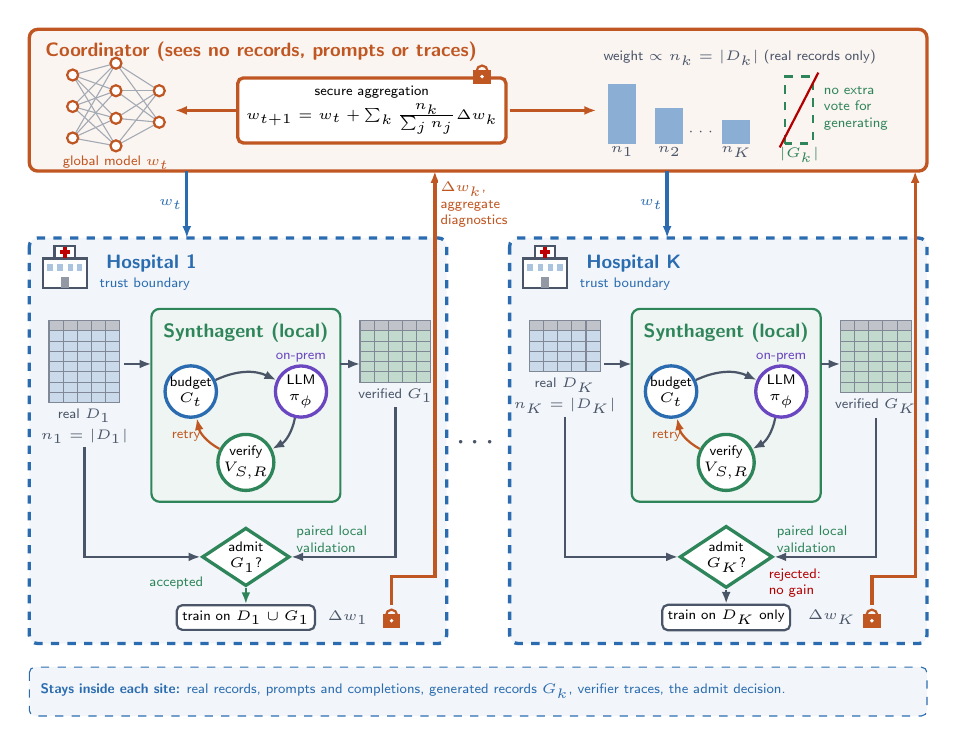
\begin{tikzpicture}[
  font=\sffamily\scriptsize,
  >={Latex[length=1.5mm]},
  flow/.style={->,thick,sgray},
  down/.style={->,very thick,sblue},
  up/.style={->,very thick,sorange},
  pan/.style={rounded corners=3pt,draw=#1,very thick,fill=#1!6},
  ttl/.style={font=\sffamily\bfseries\scriptsize,text=#1},
  lab/.style={font=\sffamily\tiny,text=#1,inner sep=1pt},
  nd/.style={circle,draw=#1,very thick,fill=white,minimum size=6.5mm,inner sep=0pt,font=\sffamily\tiny,align=center},
  diam/.style={diamond,aspect=1.5,draw=sgreen,very thick,fill=white,inner sep=0.5pt,font=\sffamily\tiny,align=center},
]
%---------------------------------------------------------------- icons
\def\lock#1#2{% padlock at (#1), colour #2
  \begin{scope}[shift={(#1)}]
    \draw[#2,thick] (-0.07,0.05) arc[start angle=180,end angle=0,radius=0.07];
    \fill[#2] (-0.11,-0.11) rectangle (0.11,0.06);
    \fill[white] (0,-0.02) circle (0.025);
  \end{scope}}
\def\hospital#1{% small hospital building at (#1)
  \begin{scope}[shift={(#1)}]
    \fill[white,draw=sgray,thick] (-0.28,-0.22) rectangle (0.28,0.16);
    \fill[white,draw=sgray,thick] (-0.13,0.16) rectangle (0.13,0.32);
    \fill[red!75!black] (-0.025,0.17) rectangle (0.025,0.31);
    \fill[red!75!black] (-0.065,0.215) rectangle (0.065,0.265);
    \foreach \x in {-0.19,-0.06,0.07,0.19}{\fill[sblue!40] (\x-0.035,0.0) rectangle ++(0.07,0.09);}
    \fill[sgray!60] (-0.05,-0.22) rectangle (0.05,-0.08);
  \end{scope}}
\def\tabl#1#2#3#4{% table glyph at (#1): #2 rows, row fill #3, highlighted row #4
  \begin{scope}[shift={(#1)}]
    \fill[sgray!35] (0,0) rectangle (0.9,-0.13);
    \foreach \r in {1,...,#2}{
      \ifnum\r=#4 \fill[sorange!45] (0,-0.13*\r) rectangle (0.9,-0.13*\r-0.13);
      \else \fill[#3] (0,-0.13*\r) rectangle (0.9,-0.13*\r-0.13);\fi}
    \foreach \c in {0,0.18,...,0.73}{\draw[sgray!70] (\c,0) rectangle ++(0.18,-0.13*#2-0.13);}
    \foreach \r in {0,...,#2}{\draw[sgray!70] (0,-0.13*\r) -- (0.9,-0.13*\r);}
  \end{scope}}
%---------------------------------------------------------------- one hospital site
% #1 x-offset, #2 site index label, #3 real rows (n_k), #4 generated rows,
% #5 admit decision text, #6 admit colour
\def\site#1#2#3#4#5#6{%
\begin{scope}[shift={(#1,0)}]
  % trust boundary
  \draw[pan=sblue,dashed] (0,0) rectangle (5.3,-5.15);
  \hospital{0.45,-0.42}
  \node[ttl=sblue,anchor=west] at (0.85,-0.32) {Hospital #2};
  \node[lab=sblue,anchor=west] at (0.85,-0.58) {trust boundary};
  % private data
  \tabl{0.25,-1.05}{#3}{sblue!25}{0}
  \node[lab=sgray,anchor=north] at (0.7,-1.05-0.13*#3-0.17) {real $D_#2$};
  \node[lab=sgray,anchor=north] at (0.7,-1.05-0.13*#3-0.42) {$n_#2=|D_#2|$};
  % local Synthagent loop
  \fill[sgreen!8,draw=sgreen,rounded corners=3pt,thick] (1.55,-0.9) rectangle (3.95,-3.35);
  \node[ttl=sgreen,anchor=north] at (2.75,-0.95) {\system{} (local)};
  \node[nd=sblue]  (b#2) at (2.05,-1.95) {budget\\$C_t$};
  \node[nd=spurple](l#2) at (3.45,-1.95) {LLM\\$\pi_\phi$};
  \node[nd=sgreen] (v#2) at (2.75,-2.85) {verify\\$V_{S,R}$};
  \draw[flow,bend left=25] (b#2) to (l#2);
  \draw[flow,bend left=25] (l#2) to (v#2);
  \draw[->,thick,sorange,bend left=25] (v#2) to node[lab=sorange,left,pos=.5]{retry} (b#2);
  \node[lab=spurple,anchor=south] at (3.45,-1.62) {on-prem};
  \draw[flow] (1.2,-1.6) -- (1.55,-1.6);
  % generated rows
  \tabl{4.2,-1.05}{#4}{sgreen!30}{0}
  \node[lab=sgray,anchor=north] at (4.65,-1.05-0.13*#4-0.17) {verified $G_#2$};
  \draw[flow] (3.95,-1.6) -- (4.2,-1.6);
  % admission gate
  \node[diam] (g#2) at (2.75,-4.05) {admit\\$G_#2$?};
  \draw[flow] (4.65,-1.05-0.13*#4-0.45) |- (g#2.east);
  \draw[flow] (0.7,-1.05-0.13*#3-0.7) |- (g#2.west);
  \node[lab=sgreen,anchor=north west,align=left] at (3.35,-3.62) {paired local\\validation};
  % local training and protected update
  \node[draw=sgray,thick,fill=white,rounded corners=2pt,font=\sffamily\tiny,align=center,inner sep=2pt]
       (t#2) at (2.75,-4.82) {train on #5};
  \draw[flow,#6] (g#2.south) -- (t#2.north);
  \node[lab=sgray,anchor=west] at (3.75,-4.82) {$\Delta w_#2$};
  \lock{4.6,-4.84}{sorange}
\end{scope}}
%================================================================ coordinator
\draw[pan=sorange] (0,2.65) rectangle (11.4,0.85);
\node[ttl=sorange,anchor=north west] at (0.08,2.62) {Coordinator (sees no records, prompts or traces)};
% global model glyph
\begin{scope}[shift={(0.55,1.12),yscale=0.85}]
  \foreach \i/\y in {1/0.15,2/0.55,3/0.95}{\coordinate (a\i) at (0,\y);}
  \foreach \i/\y in {1/0.05,2/0.4,3/0.75,4/1.1}{\coordinate (h\i) at (0.55,\y);}
  \foreach \i/\y in {1/0.35,2/0.75}{\coordinate (o\i) at (1.1,\y);}
  \foreach \a in {1,2,3}{\foreach \h in {1,2,3,4}{\draw[sgray!50] (a\a)--(h\h);}}
  \foreach \h in {1,2,3,4}{\foreach \o in {1,2}{\draw[sgray!50] (h\h)--(o\o);}}
  \foreach \p in {a1,a2,a3,h1,h2,h3,h4,o1,o2}{\fill[white,draw=sorange,thick] (\p) circle (0.07);}
  \node[lab=sorange,anchor=north] at (0.55,-0.04) {global model $w_t$};
\end{scope}
% secure aggregation
\node[draw=sorange,very thick,fill=white,rounded corners=2pt,align=center,inner sep=3pt,font=\sffamily\tiny]
  (agg) at (4.35,1.62) {secure aggregation\\[1pt]
  $w_{t+1}=w_t+\sum_k \frac{n_k}{\sum_j n_j}\Delta w_k$};
\lock{5.75,2.07}{sorange}
\draw[flow,sorange] (agg.west) -- (1.85,1.62);
% weights bars
\begin{scope}[shift={(7.35,1.2)}]
  \node[lab=sgray,anchor=south west] at (-0.1,0.95) {weight $\propto n_k=|D_k|$ (real records only)};
  \fill[sblue!55] (0,0) rectangle (0.35,0.75);   \node[lab=sgray,anchor=north] at (0.18,0) {$n_1$};
  \fill[sblue!55] (0.6,0) rectangle (0.95,0.45); \node[lab=sgray,anchor=north] at (0.78,0) {$n_2$};
  \fill[sblue!55] (1.45,0) rectangle (1.8,0.3);  \node[lab=sgray,anchor=north] at (1.63,0) {$n_K$};
  \node[lab=sgray] at (1.2,0.15) {$\cdots$};
  % ghost bar: generated rows do not count
  \draw[sgreen,dashed,thick] (2.25,0) rectangle (2.6,0.85);
  \draw[red!70!black,thick] (2.18,-0.05) -- (2.67,0.9);
  \node[lab=sgreen,anchor=north,align=center] at (2.43,0) {$|G_k|$};
  \node[lab=sgreen,anchor=west,align=left] at (2.7,0.45) {no extra\\vote for\\generating};
\end{scope}
\draw[flow,sorange] (6.1,1.62) -- (7.2,1.62);
%================================================================ sites
\site{0}{1}{7}{5}{$D_1\cup G_1$}{sgreen}
\node[font=\sffamily\bfseries\large,text=sgray] at (5.7,-2.6) {$\cdots$};
\site{6.1}{K}{4}{6}{$D_K$ only}{sgray}
\node[lab=red!70!black,anchor=west,align=left] at (6.1+3.25,-4.38) {rejected:\\no gain};
\node[lab=sgreen,anchor=east,align=right] at (2.25,-4.38) {accepted};
%================================================================ boundary crossings
\draw[down] (2.0,0.85) -- node[lab=sblue,left,align=right]{$w_t$} (2.0,0.0);
\draw[up]   (4.6,-4.66) -- (4.6,-4.3) -- (5.15,-4.3) -- (5.15,0.0) -- (5.15,0.85);
\draw[down] (8.1,0.85) -- node[lab=sblue,left,align=right]{$w_t$} (8.1,0.0);
\draw[up]   (6.1+4.6,-4.66) -- (6.1+4.6,-4.3) -- (6.1+5.15,-4.3) -- (6.1+5.15,0.85);
\node[lab=sorange,anchor=west,align=left,fill=white] at (5.18,0.42) {$\Delta w_k$,\\aggregate\\diagnostics};
%================================================================ legend
\begin{scope}[shift={(0,-5.45)}]
  \fill[sblue!6,draw=sblue,dashed,rounded corners=2pt] (0,0) rectangle (11.4,-0.62);
  \node[lab=sblue,anchor=west,align=left] at (0.1,-0.31)
    {\textbf{Stays inside each site:} real records, prompts and completions, generated records $G_k$, verifier traces, the admit decision.};
\end{scope}
\end{tikzpicture}
}
\end{minipage}\hfill
\begin{minipage}[c]{0.37\textwidth}
\caption{Deployment across healthcare facilities. Each healthcare facility runs \system (context selection, a locally served LLM, validation and correction) inside its own infrastructure, then decides with paired local validation whether to use the synthetic records $G_k$ (Facility~1) or to train on real data only (Facility~$K$). Only the model update $\Delta w_k$ and approved aggregate diagnostics leave the healthcare facility. The coordinator weights each update by the number of real records $n_k=|D_k|$ (Equation~\eqref{eq:federated-aggregate}), so generating more records gives a healthcare facility no extra weight.}
\label{fig:federated}
\end{minipage}
\end{figure*}

%======================================================================
\section{Experimental Setup}
\label{sec:setup}
%======================================================================
The system guarantees R1--R3 by construction; R4--R6 must be measured, and in small data measuring them reliably is itself a challenge. This section describes the data, the protocol and the measures with which we answer RQ1--RQ4, and explains why each choice was made.

\subsection{Datasets}
We use healthcare data because small data is most common there and because the case for SDG, more training records without exposing patients, is strongest~\cite{rieke2020digitalhealth}. We use public datasets so that every result can be reproduced. Table~\ref{tab:datasets} lists the six classification datasets: five from the UCI repository~\cite{uciheart,ucibreast,uciheartfailure,uciilpd,uciparkinsons} and the Pima Indians diabetes benchmark~\cite{smith1988diabetes}. They are widely used, each has fewer training records than the minimum sample size recommended for its task by the criteria of Riley et al.~\cite{riley2019binary} (ratio $n^{\star}/n_{\mathrm{tr}}\ge1$), and together they span the factors that make small data harder: 195 to 768 records, 8 to 30 features, two to five classes, a smallest class from 4.3\% to 37.3\% of the records, and ratios between 1.0 and 42.1. We keep the original five-class heart-disease target and impute the few missing values (0.1\% of the cells in two datasets) with the mean for numerical and the mode for categorical features.

\begin{table}[t]
\centering
\caption{Evaluation datasets. $n$: records; $d$: features; $k$: classes; $n_{\min}$: records in the smallest class; $n^{\star}$: minimum sample size by the first criterion of Riley et al.~\cite{riley2019binary} (shrinkage 0.9, $d(k-1)$ parameters, anticipated $R^2_{\mathrm{CS}}$ of 15\% of its maximum); Ratio: $n^{\star}/n_{\mathrm{tr}}$, with $n_{\mathrm{tr}}=0.8n$ the training size.}
\label{tab:datasets}
\footnotesize
\setlength{\tabcolsep}{3pt}
\begin{tabular*}{\columnwidth}{@{\extracolsep{\fill}}lrrrrrr@{}}
\toprule
Dataset & $n$ & $d$ & $k$ & $n_{\min}$ (\%) & $n^{\star}$ & Ratio \\
\midrule
Heart disease & 303 & 13 & 5 & 13 (4.3) & 10,201 & 42.1 \\
Breast cancer & 569 & 30 & 2 & 212 (37.3) & 2,302 & 5.1 \\
Heart failure & 299 & 12 & 2 & 96 (32.1) & 946 & 4.0 \\
Diabetes & 768 & 8 & 2 & 268 (34.9) & 621 & 1.0 \\
Liver disease & 583 & 10 & 2 & 167 (28.6) & 808 & 1.7 \\
Parkinson's & 195 & 22 & 2 & 48 (24.6) & 1,851 & 11.9 \\
\bottomrule
\end{tabular*}
\par\vspace{2pt}\raggedright\scriptsize For heart disease, $n^{\star}$ applies the binary criterion to the smallest class versus the rest and is an approximation. Parkinson's contains several recordings per subject, so its effective number of independent records is lower and its ratio higher than shown.
\end{table}

\subsection{Protocol}
Measuring whether synthetic records help a classifier requires real records that the generator has never seen, so each dataset is split into a training partition, given to the generator, and a test partition, used only to score classifiers. A single split, however, is unreliable in small data: the test partition holds only 39 to 154 records, and the result changes with the split. We therefore repeat the split ten times with seeds 43 to 52 (80/20 holdouts) and report means and standard deviations. In each repetition the generator receives the training partition and produces as many synthetic records as there are training records; the LLM sees a 20\% sample of the training partition as context and generates at temperature 0.3, a value fixed in advance to favour adherence to the output format while keeping some diversity.

The utility of synthetic data also depends on the learner: interpolated records can help a nearest-neighbour classifier and harm a boosted ensemble. To avoid conclusions tied to one learner, we train ten classifiers that cover the main model families: linear (logistic regression, LR), kernel (support vector machine, SVM), distance-based ($k$-nearest neighbours, $k$NN), probabilistic (Gaussian naive Bayes, NB), a single tree (decision tree, DT), bagging (random forest, RF), boosting (gradient boosting, GB; AdaBoost; XGBoost) and a neural network (multilayer perceptron, MLP). Each classifier is trained in three regimes and scored on the same test partition: real records only, synthetic records only, and real plus synthetic records. XGBoost failed on liver disease in every repetition because the labels are coded $\{1,2\}$; the code now re-encodes them, but filling this cell would require regenerating every configuration, so we report 59 of 60 classifier--dataset cells.

\subsection{Configurations}
We evaluate 14 configurations and analyse only those that completed all six datasets and ten repetitions. The first group answers RQ1. A \emph{direct-prompting} baseline uses the same prompts and context as \system but none of its control layer: the response is parsed with a strict JSON parser, and there is no repair, schema mapping, correction, retry or completion loop. Seven \emph{control-layer variants} then change one element of the pipeline at a time: the reference \system; three variants that disable a component (type rules, post-processing, and a legacy context-join option); dense and diverse context selection; and a variant in which the LLM chooses context size, selection strategy and temperature from a profile of the dataset. All eight use GPT-4o mini, the least expensive LLM, so that every comparison runs at the lowest cost.

The second group answers RQ4. Four \emph{LLMs} run the reference configuration: GPT-4o mini, GPT-4.1 mini, GPT-4o and GPT-4.1, a $2\times2$ design that crosses model generation (4o versus 4.1) with model size (mini versus full). Drawing them from one provider keeps the interface, tokenizer and output mode constant, so that differences can be attributed to the model; the control layer itself works with any OpenAI-compatible endpoint, including locally served open models. Three \emph{established generators} use the same splits: SMOTE~\cite{chawla2002smote}, which balances every class to the majority count and therefore emits only non-majority records, and CTGAN and TVAE~\cite{xu2019ctgan} with the default settings of the reference implementation (300 epochs). In total, the 14 configurations give 840 dataset--configuration runs and up to 25,200 classifier fits.

Three of the control-layer variants turn out to change nothing in this setting. With no user rules, disabling post-processing removes a step that does nothing; the context-join option affects only a legacy fidelity score; and disabling type rules cannot change the output because the validator never found a violation with GPT-4o mini. Together with the reference, these variants are therefore four independent runs of the same pipeline, and we use them as such: their spread estimates the variation between repeated runs, which we call the \emph{noise floor}. A difference between two configurations that is smaller than this spread is not evidence of an effect.

\subsection{Measures}
Each requirement of the problem statement has its own measure. For \emph{reliability} (R1--R3), we record the number of records delivered against the number requested, the number of malformed responses, completeness (the percentage of non-empty values), the corrections made by the control layer and the cost in tokens and generation time. For \emph{fidelity} (R4), we compare the synthetic records alone, without the real context, with the real training records over the numerical features $\mathcal{J}$:
\begin{equation}
\begin{aligned}
F_{\mathrm{JSD}}&=100\Bigl(1-\tfrac{1}{|\mathcal{J}|}
\textstyle\sum_{j\in\mathcal{J}}D_{\mathrm{JS}}(D_j,G_j)\Bigr),\\
F_{\mathrm{corr}}&=100\bigl(1-\operatorname{mean}|\Sigma_D-\Sigma_G|\bigr),
\end{aligned}
\label{eq:fidelity}
\end{equation}
where $D_{\mathrm{JS}}$ is the Jensen--Shannon divergence between real and synthetic marginals and $\Sigma_D$, $\Sigma_G$ are their correlation matrices; both scores equal 100 for identical distributions. We add a classifier two-sample test (C2ST)~\cite{lopezpaz2017c2st}, in which a random forest is trained to separate real from synthetic records and an accuracy close to 0.5 means they are hard to tell apart, and, for the established generators and direct prompting, the percentage of \emph{valid} records, whose values lie in the observed ranges and categories and are integers where the real feature is, a stricter criterion than R2, which concerns features and types only. For \emph{privacy} (R5), a membership-inference attack scores each real record by its distance to the nearest synthetic record and reports the ROC AUC between training and test records, where 0.5 is chance. For \emph{utility} (R6), the paired change for metric $m\in\{\mathrm{accuracy},\mathrm{F1}\}$, dataset $d$, classifier $c$ and repetition $h$ is
\begin{equation}
\Delta m_{d,c,h}=m\bigl(D^{\mathrm{tr}}_{d,h}\cup G_{d,h};\,c\bigr)-m\bigl(D^{\mathrm{tr}}_{d,h};\,c\bigr),
\label{eq:utility}
\end{equation}
with both models scored on the same test partition, so that variation between test partitions is not mistaken for an effect of SDG. We use binary F1 for the binary tasks and class-weighted F1 for heart disease; binary F1 scores the class coded 1, which is the minority class for heart failure and diabetes and the majority class for liver disease and Parkinson's. Changes are reported in percentage points (pp).

\subsection{Statistical Analysis}
Repetitions and classifiers are not independent datasets, so we average them within each dataset and treat the six datasets as matched blocks. Configurations are compared with the Friedman test,
\begin{equation}
\chi^2_F=\frac{12M}{Q(Q+1)}\sum_{a=1}^{Q}\bar{\mathrm{rk}}_a^{\,2}-3M(Q+1),
\label{eq:friedman}
\end{equation}
where $\bar{\mathrm{rk}}_a$ is the average rank of configuration $a$ over $M=6$ datasets and $Q$ the number of configurations, followed by two-sided Wilcoxon signed-rank tests of the best-ranked configuration against every other, with Holm correction~\cite{demsar2006statistical,holm1979procedure}. Per-cell tests of augmented versus real-only training over the ten repetitions are Holm-corrected within each metric. With six blocks the tests have limited power, which is precisely why we report effect sizes and the noise floor alongside $p$-values. With these measures in place, we can now answer the research questions in order.

%======================================================================
\section{Results}
\label{sec:results}
%======================================================================
\subsection{RQ1: What the Control Layer Delivers}
\label{sec:rq1}
The first question is whether the control layer is needed at all, and the direct-prompting baseline answers it. Table~\ref{tab:raw} compares it with the reference \system, both with GPT-4o mini, on the same prompts, context and splits. Direct prompting returned the requested number of records in none of the 60 runs. It fell short in 50 runs, by 4\% to 43\%, and overshot in the 10 diabetes runs, by up to 3.4\%. On average it delivered 87.6\% of the requested records, and as little as 64.0\% on the 30-feature breast-cancer dataset, where the model often returned fewer than the 30 records requested per batch. Ten responses, eight on breast cancer and two on Parkinson's, were not valid JSON and lost an entire batch each. \system delivers exactly the requested number by construction, because its completion loop requests the missing records and truncates any excess, and its parser recovers malformed responses instead of discarding them.

\begin{table}[t]
\centering
\caption{Direct prompting versus \system (RQ1), both with GPT-4o mini, over ten splits. Delivered: records returned as a percentage of those requested (range over splits); Malf.: malformed responses; $\Delta$F1: mean F1 change (pp).}
\label{tab:raw}
\scriptsize
\setlength{\tabcolsep}{2pt}
\begin{tabular*}{\columnwidth}{@{\extracolsep{\fill}}lrrrrrr@{}}
\toprule
& & \multicolumn{3}{c}{Direct prompting} & \multicolumn{2}{c}{\system} \\
\cmidrule(lr){3-5}\cmidrule(l){6-7}
Dataset & $N$ & Delivered (\%) & Malf. & $\Delta$F1 & Delivered & $\Delta$F1 \\
\midrule
Heart disease & 242 & 93.5 (91.7--94.6) & 0 & $-0.15$ & 100 & $-0.97$ \\
Breast cancer & 455 & 64.0 (56.9--69.0) & 8 & $-0.78$ & 100 & $-0.62$ \\
Heart failure & 239 & 94.5 (93.3--95.8) & 0 & $+0.26$ & 100 & $-1.00$ \\
Diabetes & 614 & 102.2 (101.3--103.4) & 0 & $+2.23$ & 100 & $+2.39$ \\
Liver disease & 466 & 93.8 (92.7--95.5) & 0 & $+0.12$ & 100 & $+0.13$ \\
Parkinson's & 156 & 77.3 (62.2--87.8) & 2 & $-1.94$ & 100 & $-0.77$ \\
\midrule
Mean & & 87.6 & 10 & $-0.04$ & 100 & $-0.14$ \\
\bottomrule
\end{tabular*}
\end{table}

The control layer achieves this without changing the quality of the records. The two configurations have the same marginal fidelity (JSD 72.7), similar correlation preservation (71.2 versus 72.6) and C2ST accuracy (0.883 versus 0.878), a membership AUC near chance (0.517 versus 0.526) and mean utility changes within the noise floor estimated below ($-1.36$ versus $-1.19$ pp in accuracy, $-0.04$ versus $-0.14$ pp in F1). The direct responses contained no type errors or unknown features with this LLM, so its failures were failures of volume and syntax, exactly the ones the completion loop and the parser address. The cost of the control layer is small: 73,510 tokens per repetition against 72,126, or 1.9\% more. The two configurations differ, in other words, not in what the records look like but in whether the user receives the dataset that was requested.

Having established that the control layer is needed, we ask which of its design choices change the outcome. Table~\ref{tab:ablation} compares the seven control-layer variants. The first four rows run the same pipeline, so their spread is the noise floor: JSD 72.43--72.92, correlation 70.83--72.93, mean accuracy change $-1.80$ to $-1.19$ pp, mean F1 change $-0.18$ to $+0.28$ pp and attack AUC 0.523--0.534. Differences of about 0.5 JSD points, 2 correlation points or 0.6 pp of utility between two runs are therefore not evidence of a design effect. The same rows show that generation time is a poor cost measure: the four equivalent runs take 228 to 379 seconds per repetition, depending on the provider, while their token counts differ by less than 2\%. We therefore measure cost in tokens.

\begin{table*}[t]
\centering
\caption{Control-layer variants (RQ1), all with GPT-4o mini. The first four rows run the same pipeline and define the noise floor. Seconds and tokens are means per repetition. Bold: best value among the LLM configurations; lower is better for C2ST, for the distance of the attack AUC from 0.5, and for cost.}
\label{tab:ablation}
\footnotesize
\begin{tabular*}{\textwidth}{@{\extracolsep{\fill}}lrrrrrrrr@{}}
\toprule
& \multicolumn{4}{c}{Fidelity (R4) and privacy (R5)} & \multicolumn{2}{c}{Utility change (R6, pp)} & \multicolumn{2}{c}{Cost per repetition (R3)} \\
\cmidrule(lr){2-5}\cmidrule(lr){6-7}\cmidrule(l){8-9}
Configuration & JSD & Corr. & C2ST & Attack AUC & Acc. & F1 & Seconds & Tokens \\
\midrule
\multicolumn{9}{l}{\textit{Noise floor: four runs of the same pipeline}}\\
Reference \system & 72.70 & 72.57 & 0.878 & 0.526 & \best{$-1.19$} & $-0.14$ & 378.7 & 73,510 \\
No type rules & 72.92 & 72.93 & 0.876 & 0.534 & $-1.80$ & $-0.04$ & 321.6 & \best{72,188} \\
No post-processing & 72.43 & 70.83 & 0.883 & \best{0.523} & $-1.71$ & \best{$+0.28$} & 251.5 & 72,235 \\
No context join & 72.52 & 71.18 & 0.880 & 0.531 & $-1.31$ & $-0.18$ & \best{228.1} & 72,576 \\
\midrule
\multicolumn{9}{l}{\textit{Design choices}}\\
Dense context & 72.87 & 70.88 & 0.878 & 0.525 & $-1.24$ & $+0.07$ & 238.8 & 72,600 \\
Diverse context & \best{73.27} & \best{73.72} & \best{0.872} & 0.544 & $-1.34$ & $-0.13$ & 271.1 & 73,757 \\
LLM-chosen settings & 72.53 & 70.10 & 0.886 & 0.526 & $-1.25$ & $+0.11$ & 310.2 & 115,245 \\
\bottomrule
\end{tabular*}
\end{table*}

Against this floor, the design choices have small effects. Dense context stays inside the floor on every measure. Diverse context is the only choice that leaves it on fidelity, with the highest JSD (73.27) and correlation (73.72) and the lowest C2ST accuracy (0.872), but also the highest attack AUC (0.544): records that cover more of the feature space lie closer to more real records. Letting the LLM choose its own settings stays inside the floor on fidelity and utility and costs 57\% more tokens (115,245 versus 73,510). The Friedman tests find no difference in utility between the variants ($\chi^2_F(7)=3.10$, $p=.875$ for accuracy; $\chi^2_F(7)=4.39$, $p=.734$ for F1), and every Holm-adjusted comparison has $p=1.0$. The ranks in Figure~\ref{fig:ranks} show how little the variants separate: LLM-chosen settings rank best on accuracy (3.75), and the no-post-processing variant, which changes nothing, ranks best on F1 (3.33). SMOTE ranks sixth of eight on accuracy (5.00) and second on F1 (3.67).

\begin{figure}[t]
\centering
\assetfigure{\columnwidth}{generated/architecture_ranks.pdf}
\caption{Average ranks of the control-layer variants and SMOTE over the six datasets (lower is better). Neither accuracy nor F1 shows a significant difference.}
\label{fig:ranks}
\end{figure}

The correction steps were rarely needed with GPT-4o mini: it produced no type violation, and the local parser fixed every defect in its responses without a repair request. They were needed with GPT-4.1 mini, the fastest LLM we tested, which produced on average 7.4 type violations per repetition on breast cancer and one malformed response in ten repetitions on diabetes. These were detected and sent back for correction instead of entering the dataset, and the resulting datasets were complete and gave the best mean accuracy change of all configurations (Table~\ref{tab:backend}). A faster but less disciplined model can thus be used safely, because its failures are caught. Across all LLMs, the synthetic datasets have 99.7\% (GPT-4o mini) to 100.0\% of their values filled.

\noindent\textit{Answer to RQ1.} The control layer is what makes LLM output usable as a dataset: direct prompting never returned the requested size and lost whole batches to malformed responses, whereas \system delivers complete datasets of the requested size, records its cost and catches the failures of less disciplined models, for 1.9\% more tokens. Within one LLM, no design choice moves fidelity or utility beyond the noise floor, except a small fidelity gain from diverse context. The value of the control layer lies in reliability rather than in a higher score, which leads to the next question: how good are the records it delivers?

\subsection{RQ2: Fidelity and Privacy}
\label{sec:rq2}
Table~\ref{tab:full} reports the reference configuration per dataset. Marginal fidelity averages 72.7 out of 100, from 65.2 on the five-class heart-disease dataset, the furthest below its required sample size (ratio 42.1), to 80.2 on diabetes, the closest to it (ratio 1.0). The membership-inference attack stays near chance, at 0.526 on average and at most 0.567 on any dataset, so the synthetic records do not reveal which real records were used; this is a diagnostic for one attack, not a formal guarantee. The C2ST accuracy of 0.878 shows that a classifier can still separate real from synthetic records, so we do not claim that the synthetic records can replace real ones.

\begin{table}[t]
\centering
\caption{Reference configuration (GPT-4o mini) per dataset, averaged over ten repetitions and all classifiers (RQ2, RQ3). JSD and correlation are on a 0--100 scale.}
\label{tab:full}
\footnotesize
\setlength{\tabcolsep}{2.2pt}
\begin{tabular*}{\columnwidth}{@{\extracolsep{\fill}}lrrrrrrrr@{}}
\toprule
& \multicolumn{4}{c}{R4 and R5} & \multicolumn{2}{c}{Acc.\ (\%)} & \multicolumn{2}{c}{Change (pp)} \\
\cmidrule(lr){2-5}\cmidrule(lr){6-7}\cmidrule(l){8-9}
Dataset & JSD & Corr. & C2ST & AUC & Real & Aug. & Acc. & F1 \\
\midrule
Breast & 77.2 & 74.5 & 0.911 & 0.550 & 95.1 & 94.4 & $-0.66$ & $-0.62$ \\
Diabetes & 80.2 & 44.0 & 0.897 & 0.504 & 74.2 & 74.1 & $-0.03$ & $+2.39$ \\
Heart dis. & 65.2 & 76.6 & 0.893 & 0.507 & 56.6 & 53.4 & $-3.15$ & $-0.97$ \\
Heart fail. & 71.2 & 81.2 & 0.892 & 0.534 & 74.1 & 71.6 & $-2.53$ & $-1.00$ \\
Liver & 71.8 & 73.8 & 0.883 & 0.495 & 67.4 & 67.6 & $+0.19$ & $+0.13$ \\
Parkinson's & 70.6 & 85.3 & 0.789 & 0.567 & 84.9 & 84.0 & $-0.97$ & $-0.77$ \\
\midrule
Mean & 72.7 & 72.6 & 0.878 & 0.526 & 75.4 & 74.2 & $-1.19$ & $-0.14$ \\
\bottomrule
\end{tabular*}
\end{table}

\noindent\textit{Answer to RQ2.} The synthetic records follow the real marginals reasonably well without reproducing the real records, but they remain distinguishable from real data. Whether records of this quality help a classifier is the next question.

\subsection{RQ3: Utility for Classifiers Trained on Small Data}
\label{sec:rq3}
Any utility effect must be judged against how much classifiers trained on real data alone already vary, so we measure that first (Table~\ref{tab:baselines}). The variation is large. On the 195-record Parkinson's dataset, MLP accuracy is $72.3\pm18.2\%$, while tree ensembles exceed 92\%. On heart failure, SVM and $k$NN reach 63.3\% and 61.3\% accuracy but an F1 of only 0.0 and 0.7, because they almost never predict the minority class; accuracy alone would hide the very failure that SDG is meant to address.

\begin{table*}[t]
\centering
\caption{Real-only baselines (RQ3) over ten 80/20 splits: mean in percent, standard deviation in small type. XGBoost on liver disease (--) failed in every split because the labels are coded $\{1,2\}$.}
\label{tab:baselines}
\footnotesize
\setlength{\tabcolsep}{2pt}
\begin{tabular*}{\textwidth}{@{\extracolsep{\fill}}lrrrrrrrrrrrr@{}}
\toprule
 & \multicolumn{2}{c}{Heart dis.} & \multicolumn{2}{c}{Breast} & \multicolumn{2}{c}{Heart fail.} & \multicolumn{2}{c}{Diabetes} & \multicolumn{2}{c}{Liver} & \multicolumn{2}{c}{Parkinson's} \\
\cmidrule(lr){2-3} \cmidrule(lr){4-5} \cmidrule(lr){6-7} \cmidrule(lr){8-9} \cmidrule(lr){10-11} \cmidrule(lr){12-13}
Classifier & Acc. & F1 & Acc. & F1 & Acc. & F1 & Acc. & F1 & Acc. & F1 & Acc. & F1 \\
\midrule
RF & 61.0\sd{4.4} & 57.0\sd{5.9} & 95.6\sd{1.8} & 95.0\sd{2.8} & 84.3\sd{3.3} & 76.8\sd{4.4} & 74.9\sd{2.8} & 60.4\sd{6.0} & 71.1\sd{3.5} & 81.4\sd{2.4} & 92.3\sd{3.2} & 94.8\sd{2.2} \\
DT & 53.4\sd{3.9} & 54.0\sd{5.0} & 93.3\sd{2.3} & 92.1\sd{4.0} & 79.2\sd{4.7} & 68.4\sd{9.2} & 71.1\sd{3.8} & 57.2\sd{6.4} & 66.0\sd{3.2} & 76.3\sd{3.1} & 85.1\sd{5.6} & 89.7\sd{3.8} \\
MLP & 56.6\sd{6.4} & 52.5\sd{7.6} & 94.7\sd{0.9} & 94.0\sd{2.1} & 48.3\sd{12.9} & 34.2\sd{24.7} & 68.4\sd{4.1} & 52.9\sd{12.0} & 68.4\sd{4.1} & 79.4\sd{3.6} & 72.3\sd{18.2} & 77.8\sd{26.1} \\
SVM & 54.8\sd{6.8} & 39.0\sd{7.9} & 93.3\sd{2.1} & 92.4\sd{3.4} & 63.3\sd{5.2} & 0.0\sd{0.0} & 75.6\sd{2.2} & 57.3\sd{4.7} & 70.7\sd{2.9} & 82.8\sd{2.0} & 81.0\sd{8.2} & 88.5\sd{5.2} \\
LR & 59.8\sd{5.6} & 56.5\sd{5.0} & 95.2\sd{2.0} & 94.6\sd{2.6} & 80.5\sd{3.6} & 68.9\sd{8.4} & 77.3\sd{2.0} & 62.8\sd{5.4} & 70.3\sd{4.0} & 81.1\sd{3.2} & 86.9\sd{5.6} & 91.3\sd{3.9} \\
kNN & 55.4\sd{6.3} & 44.4\sd{7.9} & 94.3\sd{1.8} & 93.4\sd{3.2} & 61.3\sd{4.1} & 0.7\sd{2.1} & 75.5\sd{1.8} & 60.0\sd{3.3} & 68.6\sd{4.2} & 79.7\sd{3.2} & 83.6\sd{5.6} & 89.5\sd{3.9} \\
NB & 55.7\sd{5.3} & 56.9\sd{5.0} & 93.9\sd{1.7} & 93.1\sd{3.2} & 75.0\sd{4.9} & 56.7\sd{13.1} & 76.4\sd{2.4} & 64.0\sd{4.9} & 55.9\sd{3.7} & 55.9\sd{3.8} & 71.5\sd{4.4} & 76.6\sd{4.0} \\
GB & 54.1\sd{5.5} & 52.8\sd{6.3} & 95.9\sd{2.2} & 95.4\sd{2.8} & 83.0\sd{4.9} & 75.4\sd{7.2} & 74.7\sd{3.0} & 61.7\sd{5.8} & 67.9\sd{3.3} & 78.7\sd{2.4} & 92.1\sd{4.0} & 94.7\sd{2.6} \\
AdaBoost & 60.8\sd{7.6} & 60.7\sd{7.3} & 97.1\sd{1.5} & 96.8\sd{1.7} & 82.5\sd{3.0} & 74.2\sd{6.5} & 74.9\sd{2.2} & 60.8\sd{4.7} & 67.4\sd{3.4} & 78.2\sd{3.3} & 91.3\sd{3.8} & 94.2\sd{2.5} \\
XGBoost & 54.3\sd{4.6} & 52.0\sd{5.1} & 97.2\sd{1.4} & 96.9\sd{1.8} & 83.5\sd{4.0} & 75.5\sd{7.0} & 72.7\sd{2.8} & 59.1\sd{6.2} & \multicolumn{1}{c}{--} & \multicolumn{1}{c}{--} & 93.3\sd{5.2} & 95.6\sd{3.2} \\
\bottomrule
\end{tabular*}

\end{table*}

Against this background, the effect of synthetic records depends on both the dataset and the classifier (Table~\ref{tab:full}, Figure~\ref{fig:heatmap}). With the reference configuration, accuracy improves in 18 of 59 classifier--dataset cells, decreases in 38 and is unchanged in three; F1 improves in 26, decreases in 31 and is unchanged in two. The largest gains occur where real-only training fails on the minority class: $k$NN on heart failure, with a real-only F1 of 0.7\%, gains 15.3 F1 points, and MLP on Parkinson's, the most unstable baseline, gains 8.2 accuracy points. Classifiers that are already strong lose slightly. After Holm correction over 59 tests per metric, no single cell is significant at 0.05. Figure~\ref{fig:uncertainty} shows the variation between splits: the accuracy change is consistently negative on the two heart datasets and centred on zero for liver disease, and diabetes is the only dataset with a clearly positive F1 change at unchanged accuracy.

\begin{figure*}[t]
\centering
\assetfigure{\textwidth}{generated/utility_heatmap.pdf}
\caption{Change from real-only to real-plus-synthetic training for the reference configuration (RQ3), per classifier and dataset. Hatched cells (n/a) were not evaluated. The same synthetic data can help one classifier and harm another.}
\label{fig:heatmap}
\end{figure*}

\begin{figure}[t]
\centering
\assetfigure{\columnwidth}{generated/augmentation_uncertainty.pdf}
\caption{Variation between splits for the reference configuration (RQ3). Points are splits, after averaging the paired changes over classifiers; diamonds are means and bars 95\% $t$ intervals.}
\label{fig:uncertainty}
\end{figure}

\noindent\textit{Answer to RQ3.} With GPT-4o mini, synthetic records help the classifiers that fail on the minority class and slightly harm the strong ones; on average they leave F1 unchanged ($-0.14$ pp) and lower accuracy ($-1.19$ pp). This is what information theory leads one to expect: synthetic records cannot carry more information about the task than the real records and the generator's own knowledge together~\cite{cover2006elements}, so large average gains are unlikely. If the LLM is the source of that information, a stronger LLM should matter, and so should the choice between an LLM and a generator fitted to the data. RQ4 examines both.

\subsection{RQ4: Comparison with Established Generators and LLMs}
\label{sec:rq4}
The choice of LLM is the only factor whose effect exceeds the noise floor (Table~\ref{tab:backend}, Figure~\ref{fig:frontier}). All three alternatives to GPT-4o mini exceed it in accuracy change and two in F1 change. GPT-4.1 gives the highest marginal fidelity (75.72, 2.8 points above the floor) and the largest F1 gain ($+1.09$ pp); GPT-4.1 mini gives the best accuracy change ($-0.23$ pp) at the lowest generation time. The three stronger LLMs preserve pairwise correlations less well (62.8--64.3, against at least 70.83 for GPT-4o mini), so better marginals come at the cost of weaker dependencies. Across six datasets these differences are not significant ($\chi^2_F(3)=2.00$, $p=.572$ for accuracy; $\chi^2_F(3)=1.80$, $p=.615$ for F1); the closest comparison, GPT-4.1 mini against GPT-4o mini in accuracy, differs by $+0.86$ pp with $p_{\mathrm{Holm}}=.188$.

\begin{table}[t]
\centering
\caption{LLMs under the reference configuration (RQ4). Seconds and tokens are means per repetition.}
\label{tab:backend}
\footnotesize
\setlength{\tabcolsep}{3pt}
\begin{tabular*}{\columnwidth}{@{\extracolsep{\fill}}lrrrrrr@{}}
\toprule
LLM & JSD & Corr. & $\Delta$Acc. & $\Delta$F1 & Sec. & Tokens \\
\midrule
GPT-4o mini & 72.70 & \best{72.57} & $-1.19$ & $-0.14$ & 378.7 & \best{73,510} \\
GPT-4.1 mini & 73.60 & 62.82 & \best{$-0.23$} & $+0.92$ & \best{168.5} & 72,069 \\
GPT-4o & 73.95 & 64.32 & $-0.50$ & $+0.25$ & 255.2 & 80,046 \\
GPT-4.1 & \best{75.72} & 63.30 & $-0.44$ & \best{$+1.09$} & 201.7 & 80,652 \\
\bottomrule
\end{tabular*}
\end{table}

\begin{figure}[t]
\centering
\assetfigure{\columnwidth}{generated/quality_cost_frontier.pdf}
\caption{Fidelity, F1 change and token cost of the LLM configurations (RQ1, RQ4). Control-layer variants cluster inside the noise floor; the LLMs spread along fidelity and F1.}
\label{fig:frontier}
\end{figure}

How does LLM-based synthesis compare with generators fitted to the data? Table~\ref{tab:generators} places \system with GPT-4o mini and GPT-4.1 next to SMOTE, CTGAN and TVAE. No generator is best on every measure. CTGAN reaches the highest marginal fidelity (JSD 77.6), but its records are the easiest to detect (C2ST 0.936) and only 29.6\% of them are valid (1.0\% on Parkinson's). TVAE keeps 75.6\% valid records and SMOTE 85.7\%, although only 14.4\% on heart disease, where interpolation produces fractional values in integer-coded features. All five generators keep the membership attack near chance (0.503--0.532). Cost separates them sharply: SMOTE needs 0.015 seconds, TVAE and CTGAN 5.6 and 14.6 seconds of CPU time, and \system 73,000 to 81,000 tokens and several minutes of API time, with no training.

\begin{table}[t]
\centering
\caption{Generators compared on the same splits (RQ4). Valid: \% of records within the observed ranges, categories and integer types (not logged for the LLM runs, whose types are enforced by the validator). Seconds: API time for \system, CPU time otherwise.}
\label{tab:generators}
\scriptsize
\setlength{\tabcolsep}{1.5pt}
\begin{tabular*}{\columnwidth}{@{\extracolsep{\fill}}lrrrrrrrrr@{}}
\toprule
Generator & JSD & Corr. & C2ST & AUC & Valid & $\Delta$Acc. & $\Delta$F1 & Sec. & Tok. \\
\midrule
\system, 4o mini & 72.7 & 72.6 & 0.878 & 0.526 & -- & $-1.19$ & $-0.14$ & 379 & 73.5k \\
\system, 4.1 & 75.7 & 63.3 & 0.877 & 0.527 & -- & $-0.44$ & \best{$+1.09$} & 202 & 80.7k \\
SMOTE$^{\dagger}$ & 69.9 & 85.0 & 0.795 & 0.532 & \best{85.7} & $-3.08$ & $+0.33$ & \best{0.01} & 0 \\
CTGAN & \best{77.6} & 75.2 & 0.936 & \best{0.503} & 29.6 & $-1.40$ & $-3.37$ & 14.6 & 0 \\
TVAE & 71.9 & \best{85.6} & 0.868 & 0.515 & 75.6 & \best{$-0.09$} & $-0.21$ & 5.6 & 0 \\
\bottomrule
\end{tabular*}
\par\vspace{2pt}\raggedright\scriptsize $^{\dagger}$Emits only non-majority records, so its C2ST is not comparable.
\end{table}

Average changes, however, hide how much each generator can harm an individual dataset, and in small data a large loss on one dataset matters more than a small gain on average. Table~\ref{tab:robust} reports the F1 change per dataset. SMOTE gives the largest gains where the scored class is rare ($+10.91$ pp on heart failure, $+4.11$ on diabetes) but loses 8.20 pp on liver disease, where the scored class is the majority. CTGAN loses on every dataset, by up to 10.65 pp. TVAE gives the best accuracy change on average but loses 2.86 pp of F1 on heart failure. \system with GPT-4.1 has both the largest mean F1 gain ($+1.09$ pp) and the smallest worst case: it never lowers the F1 of a dataset by more than 0.53 pp, while raising it by 6.35 pp on heart failure. Across datasets, the differences between the five generators are not significant ($\chi^2_F(4)=6.80$, $p=.147$ for accuracy; $\chi^2_F(4)=5.60$, $p=.231$ for F1; every Holm-adjusted $p\ge.25$); TVAE has the best accuracy rank (2.00), and the two \system configurations share the best F1 rank (2.50).

\begin{table}[t]
\centering
\caption{Mean F1 change per dataset (pp) over ten splits and all classifiers (RQ4). \textsc{SA}: \system. Worst: largest loss on any dataset.}
\label{tab:robust}
\scriptsize
\setlength{\tabcolsep}{1pt}
\begin{tabular*}{\columnwidth}{@{\extracolsep{\fill}}lrrrrrrrr@{}}
\toprule
Generator & Heart d. & Breast & Heart f. & Diab. & Liver & Park. & Mean & Worst \\
\midrule
\textsc{SA}, 4o mini & $-0.97$ & $-0.62$ & $-1.00$ & $+2.39$ & $+0.13$ & $-0.77$ & $-0.14$ & $-1.00$ \\
\textsc{SA}, 4.1 & $-0.44$ & $-0.07$ & $+6.35$ & $+1.75$ & $-0.50$ & $-0.53$ & \best{$+1.09$} & \best{$-0.53$} \\
SMOTE & $-1.50$ & $-0.53$ & $+10.91$ & $+4.11$ & $-8.20$ & $-2.83$ & $+0.33$ & $-8.20$ \\
CTGAN & $-2.30$ & $-2.00$ & $-10.65$ & $-4.22$ & $-0.65$ & $-0.38$ & $-3.37$ & $-10.65$ \\
TVAE & $-0.73$ & $-0.88$ & $-2.86$ & $+0.89$ & $+2.21$ & $+0.10$ & $-0.21$ & $-2.86$ \\
\bottomrule
\end{tabular*}
\end{table}

\noindent\textit{Answer to RQ4.} The LLM is the main lever on quality and utility. With GPT-4.1, \system gives the largest and most consistent F1 gain of the five generators, at a higher cost than the established generators and without a significant advantage across six datasets. TVAE remains a cheap option for accuracy, and SMOTE for a known rare positive class.

%======================================================================
\section{Discussion and Limitations}
\label{sec:discussion}
%======================================================================
We set out to determine whether a control layer makes LLM-based SDG a reliable and useful option for small data, and the four answers combine into a clear picture. Reliability is achieved, and it is achieved by the control layer: the same LLM, prompted directly, never returned the dataset that was requested, whereas \system completes it by construction, records its cost and caught the failures of a less disciplined model, at almost no extra cost (RQ1). Usefulness is real but bounded: the synthetic records are faithful without reproducing real ones, yet distinguishable from them (RQ2); they help classifiers that fail on the minority class (RQ3); and with a stronger LLM they give the most consistent F1 gain among the generators compared (RQ4). No generator, however, improves utility significantly on all datasets. This is consistent with the data-processing inequality~\cite{cover2006elements}: SDG cannot replace missing patients, and its benefit is bounded by the knowledge the generator brings. Among the generators we compared, the LLM is the only one that brings such knowledge, and the control layer is what makes it usable.

These results translate into four practical recommendations. Choose the LLM first, since it is the only factor whose effect exceeds the variation between runs. Measure cost in tokens rather than time, which depends on the provider. Check the effect of synthetic records per classifier, on paired splits, before using them. And do not let the LLM choose its own settings without measuring the extra cost.

The conclusions are subject to several limitations. Only six datasets act as independent blocks, which limits the power of the tests, and the splits are not stratified. The Parkinson's dataset contains several recordings per subject without a subject identifier, so recordings of one person can appear in both partitions. Schema and value ranges are inferred once from the full dataset, which exposes test extremes to the profiler; train-only profiling would be stricter. JSD uses fixed histograms and is dominated by numerical features, and the membership attack is a single distance-based adversary, so no result establishes differential privacy~\cite{dwork2014dp}. The \system runs predate the counter of delivered records, so their size follows from the completion loop of Algorithm~\ref{alg:loop} rather than from a logged count, and the validity measure was logged only for the established generators and direct prompting (78.6\% valid records), so it is not compared with \system. The correction paths were exercised only by GPT-4.1 mini; a stress test with weaker or locally served models and stricter rules is needed to measure how often each one is needed, and in the current implementation the output of the last correction round and the records obtained in top-up rounds are not validated again. Context selection is not class-stratified, so a rare class can be missing from a prompt. All LLMs come from one provider; GPT-4.1 nano and o4-mini were started but did not complete every dataset and are excluded. CTGAN and TVAE use default settings, and tuned or diffusion-based generators may do better on some datasets. Finally, the sample-size ratios in Table~\ref{tab:datasets} rely on a default anticipated $R^2_{\mathrm{CS}}$ and are estimates.

Synthetic \DIFdelbegin \DIFdel{medical }\DIFdelend \DIFaddbegin \DIFadd{healthcare }\DIFaddend records can support development, teaching and software testing, but they must not inform diagnosis or policy without domain review, and near-chance performance against one membership attack does not justify releasing sensitive data. To support verification, the implementation, the experiment runner and the script that regenerates every table and figure from the stored results are publicly available.\footnote{TODO(authors): add the public repository URL required by the ICDE artifact policy.}

%======================================================================
\section{Conclusion}
\label{sec:conclusion}
%======================================================================
Small clinical datasets pose a dilemma for synthetic data generation. Generators fitted to the available records cannot add the information those records lack, whereas an LLM can bring knowledge from pre-training but returns text rather than a dataset. \system resolves the dilemma with a control layer that turns LLM responses into complete, validated datasets of the requested size and records their cost, without training on the target data. On six small \DIFdelbegin \DIFdel{medical }\DIFdelend \DIFaddbegin \DIFadd{healthcare }\DIFaddend datasets, direct prompting never delivered the requested dataset, while \system completes it by construction, at 1.9\% more tokens; with the larger, more recent LLM it gave the largest and most consistent F1 gain of five generators, although no generator was significantly better on every dataset. Because repeated runs of the same pipeline vary as much as most design choices, we recommend that SDG for small data be evaluated against such a noise floor. Future work will evaluate locally served LLMs, class-aware context selection and the deployment across healthcare facilities outlined in Section~\ref{sec:deployment}.

%======================================================================
\section*{Acknowledgment}
%======================================================================
This work is funded by national funds through FCT -- Foundation for Science and Technology, I.P., within the scope of the research unit UID/00326 -- Centre for Informatics and Systems of the University of Coimbra, \url{https://doi.org/10.54499/UID/00326/2025}.

\bibliographystyle{IEEEtran}
\bibliography{references}

\end{document}
